\documentclass[12pt]{article}
\usepackage{hyperref}
%\usepackage{a4wide}
\usepackage[margin=0.8in]{geometry}
\usepackage{graphicx}
\usepackage{wrapfig}
\newcommand{\lambdabar}{{\mkern0.75mu\mathchar '26\mkern -9.75mu\lambda}}
\date{}
\title{\LARGE \bf Nuclear and Particle Physics\\[5mm]Scattering}
\author{Daniel Ma\^{i}tre, IPPP, Durham University}

\newcommand{\V}[1]{\mathbf{#1}}
\newcommand{\GeV}{\,\rm{GeV}}
\newcommand{\mb}{\, \rm{mb}}
\newcommand{\barn}{\,\rm{b}}
\begin{document}
%%\lecture{8}

%%\section{Introduction}
\maketitle
To study the properties of a particle one can bombard it with other particles and analyse the distribution of the deflected particles in a similar fashion to optical or X-ray spectroscopy. 

\begin{figure}[h]
\begin{center}
  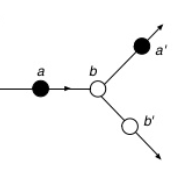
\includegraphics[scale=0.4]{images/elastic.png}
	%%\image{inelastic1.png}
 \rule{3cm}{0cm}  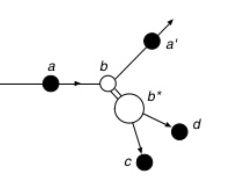
\includegraphics[scale=0.4,clip]{images/inelastic1.png} 
 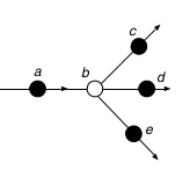
\includegraphics[scale=0.4]{images/inelastic2.png} 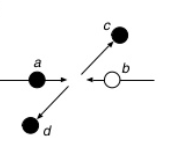
\includegraphics[scale=0.4]{images/inelastic3.png}
\end{center}
\caption{Illustration for elastic (left) and inelastic (right) scattering.}\label{fig:elasticinelastic}\end{figure}
We distinguish between
\begin{itemize}
\item \emph{elastic scattering} where the scattering particles escape unscathed from the reaction, that is they are the same particles but with different energy and momenta.
\item \emph{inelastic scattering} where at least one of the particles is changed, destroyed or more particles are created.
\end{itemize}

 The size of structures probed by a particle with momentum $p$ is given by the de-Broglie wavelength
 \[\lambdabar=\frac{\hbar}{p}=\frac{\hbar c}{\sqrt{2mc^2 E_{kin}+E_{kin}^2}}\]
The higher the energy the deeper one can ``see'' inside the structure of matter.   
%%\keypoint{The higher the energy of the projectile, the deeper one can ``see'' inside the structure of matter.}

%%\section{Cross Sections}
\section{Cross section}
The cross section for a process is the most important quantity to describe the process. To see its interpretation consider a fixed-target experiment where a beam of particles hits a target composed of scattering centres.
%%\keypoint{The cross section is a very useful quantity to characterise a physical scattering process.}
As a starting point we consider a beam of point-like particles $a$ colliding with a target of ``hard'' particles $b$ of cross-sectional area $\sigma_b$. By this we mean that if the incident particle $a$ hits the target particle $b$ within a region of area $\sigma_b$ in the plane transverse to the beam direction a collision will take place and the deflected particle $a$ will be detected as having interacted. Suppose the beam has an area $A$. If we denote the number of particles $a$ with $N_a$ then $\dot{N_a}$ is the rate of production of beam particles. The flux $\Phi_a$ is the number of particles $a$ entering the target per unit area per time unit. It can be related to the density of beam particle and their velocity by
\[\Phi_a=\frac{\dot N_a}{A}=n_a\cdot v_a\]
%%\image{beam.png}
\begin{figure}
\begin{center} 
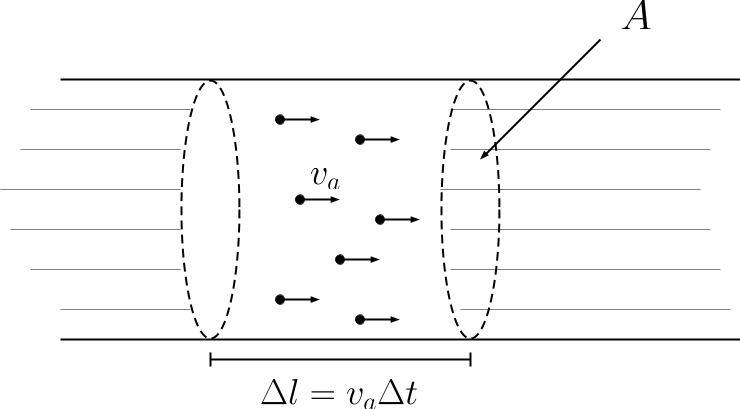
\includegraphics[scale=0.3]{images/beam.png}
\end{center}
\caption{Flux of particles of speed $v_a$ through an area $A$.}\label{fig:flux}
\end{figure}
This can be understood by counting the number of beam particles $\Delta N_a$ crossing a given area along the beam direction during a time interval $\Delta t$. It corresponds to the number of particle in the cylinder of section $A$ and height $\Delta l$ where $\Delta l$ is the distance travelled by the particles in the time $\Delta t$. So we have
\begin{equation}\label{eq:fluxa}
\Delta N_a=n_a\cdot A\cdot\Delta l=n_a \cdot A \cdot v_a\Delta t
\quad 
\Rightarrow 
\quad
\Phi_A=\frac{1}{A}\frac{\Delta N_a}{\Delta t}=n_a v_a
\end{equation}
This beam collides with a target of width $d$ containing a density $n_b$ of particles with cross-sectional area $\sigma_b$. The number of target particles available for scattering is therefore
\[N_b=n_b\cdot A\cdot d\;.\]
If $N$ is the number of collisions, the rate $\dot N$ of collisions is given by the product of the incoming flux with the area presented by the $N_b$ particles:
\begin{equation}\label{eq:ndot}
	\dot N=\Phi_a\cdot N_b\cdot \sigma_b\;.
\end{equation}
If one measures the collision rate and knows the characteristics of the beam, one can infer the area $\sigma_b$:
\[\sigma_b=\frac{\dot N}{\Phi_a\cdot N_b}\]
or in words:
\[\sigma_b=\frac{\mbox{number of reactions per time unit}}{\mbox{beam particles per unit time per unit area} \times \mbox{number of scattering centres}}\]
The denominator can be reformulated as
\[\Phi_a\cdot N_b=\frac{\dot N_a}{A} n_b\cdot A\cdot d=\dot N_a \cdot n_b\cdot d=\dot N_a \cdot \rho_b\]
where $\rho_b$ is the density of particle $b$ per unit area in the target. This way of formulating the cross section
\[\sigma_b=\frac{\mbox{number of reactions per time unit}}{\mbox{beam particles per unit time} \times \mbox{number of scattering centres per unit area}}\]
is more convenient when particle density of the beam is not constant while that of the target is.

This example was too simple because of several factors:
\begin{itemize}
\item the incoming particle can also have an ``area'' $\sigma_a$
\item the cross section can have a strong dependence on the energy
\item the effective ``cross section'' $\sigma_b$ depends on the range of the interaction, an electron would ``see'' a much larger cross section than a neutrino because the electro-magnetic force has a much larger interaction range than the weak force.
  \end{itemize}
We define the total cross section for a realistic process in the same way as for the geometric example above as:
\[\sigma_{tot}=\frac{\mbox{number of reactions per time unit}}{\mbox{beam particles per unit time} \times \mbox{number of scattering centres per unit area}}\]
which now depends on the type of particles $a$ and $b$ (which fix the interaction type) and the energy of the reaction. This includes both reactions that leave the particles $a$ and $b$ unchanged (elastic scattering) and those where new particles are created (inelastic particles).
\[\sigma_{tot}=\sigma_{el}+\sigma_{inel}\;.\]
\begin{figure}
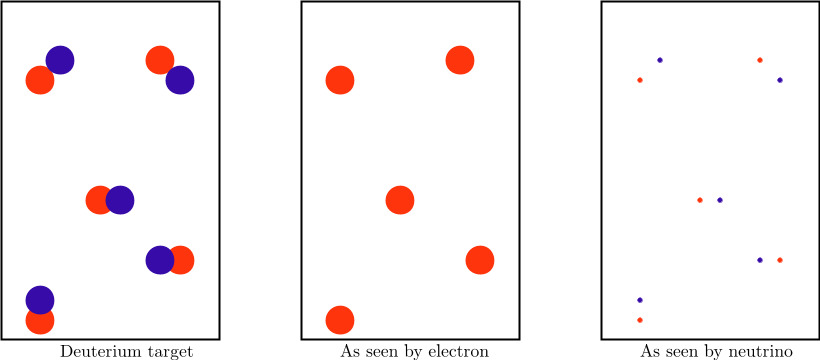
\includegraphics[scale=0.5]{images/target.png}
  \caption{Illustration of the cross section: the same target can ``look'' different depending on the particle that interacts with it. If we consider a deuterium target (left) which are composed of one proton (red) and one neutron (blue), at moderate energies an electron would mostly ``see'' the electrically charged proton (middle), while a neutron would ``see'' both the proton and the neutrino as it can interact with either, albeit with a much smaller interaction, hence the much smaller area in this illustration.}\label{fig:xsIllustration}
\end{figure}
Cross sections have the dimension of an area and are typically expressed in a unit called \emph{barn}.
\[1\, \rm{barn}= 1 \barn =10^{-28}\,m^2\]
In natural units we can express cross sections in units of inverse GeV squared:
\[1 \rm{b} \simeq 2568\,\GeV^{-2}\;,\qquad 1\GeV^{-2}=0.389\mb\]
We can separate the rate of collisions into two parts, one that is related to the experimental setup and the cross section that is a physical property of the process and independent of the details of the experimental setup:
\[\dot N = \Phi_a N_b \sigma_b\equiv \mathcal{L}\sigma_b\]
The quantity $\mathcal{L}=\Phi_aN_b=n_a v_a N_b$ is called the luminosity and has the dimensions of a flux ($m^2/s$).

A similar formula can be derived when colliding two beams. If we collide a beam with $N_a$ particles with a beam of $N_b$ particles colliding at an area $A$ with a frequency $\nu$, the luminosity is given by
\[\mathcal{L}=\frac{N_aN_b}{A}\nu\;.\]
This formula assumes a constant density of particles $a$ and $b$ in the area $A$.

In practice it is not possible to measure the total cross section, as detectors cannot cover the entire solid angle around the interaction point. We define the differential cross section $d\sigma(\theta)/d\Omega$ where $d\Omega$ is the solid angle element. Typically an experiment will measure only a fraction of the total cross section:
\[\sigma_{measured}=\int\limits_{\Omega_c}\frac{d\sigma}{d\Omega}d\Omega\]
  where $\Omega_c$ is the area the detector covers.

  The differential cross section can be differential in other observables, such as the energy of the scattered particle for example, in order to elucidate more of the properties of the scattering particles. For example one could apply a filter to the detector to only register scattered particles whose energy is between the energies $E_{min}$ and $E_{max}$. The cross section in this case would be
  \[\sigma_{measured}=\int\limits_{\Omega_c}\int\limits_{E_{min}}^{E_{max}}\frac{d\sigma}{d\Omega\,dE}dE \,d\Omega\]
Performing this measurement for different ranges of energies allows to extract information about the differential cross section $\frac{d\sigma}{d\Omega\,dE}$.
%
%%\section{Representing Cross Sections}
\section{Representing cross sections}
%
%
In most cases a cross section is represented in a differential way with respect to one or more observables. While it is possible to make a theoretical prediction for a distribution $d\sigma/d\mathcal{O}$ with respect to a continuous observable $\mathcal{O}$ it is not possible in general to measure the differential cross section at an exact value of that observable. This is because the probability of the observable being exactly that value is $0$, it is only non-vanishing if we consider the probability for the observable to be in an interval containing the value. For this reason differential cross sections are represented as \emph{histograms}. The range of values for the observable $\mathcal{O}$ is divided into intervals (called $bins$) and events with values of $\mathcal{O}$ are assigned to the bin that contains $\mathcal{O}$. 

An example of an histogram is shown in Figure~\ref{fig:histograms}. There are two ways of displaying an histogram. The first is to show the number of events in each bins. Changing the binning changes the height of the histogram bars as combining bins together results in a larger number of event in the bins. This is illustrated in the first row of Figure~ref{fig:histograms}. The second way is to normalise the number of events with the luminosity and the bin width. Doing so ensures that the shape of the histogram does not change too much as the binning changes and the histogram heights will follow the actual continuous distribution $d\sigma/d\mathcal{O}$. To obtain the theoretical prediction for the height of a bin between the values $\mathcal{O}_1$ and $\mathcal{O}_2$ one needs to integrate the differential cross section between these values:
\[h_{predicted}=\int\limits_{\mathcal{O}_1}^{\mathcal{O}_2}\frac{d\sigma}{d\mathcal{O}}d\mathcal{O}\;.\]
One can see the total cross section as a limiting case where we have only one bin covering the entire range of $\mathcal{O}$ that can be measured. When differential cross sections are reported as a function of single values of the observable and not an interval an average over an enclosing interval is implied. This could for example be set by the experimental resolution on the observable $\mathcal{O}$.   
%%\keypoint{More information about the dynamics of the interaction can be shown by measuring the cross section differentially with respect to observables. Such a differential cross section is represented as an histogram.}
\begin{figure}
%%\image{histograms.png}
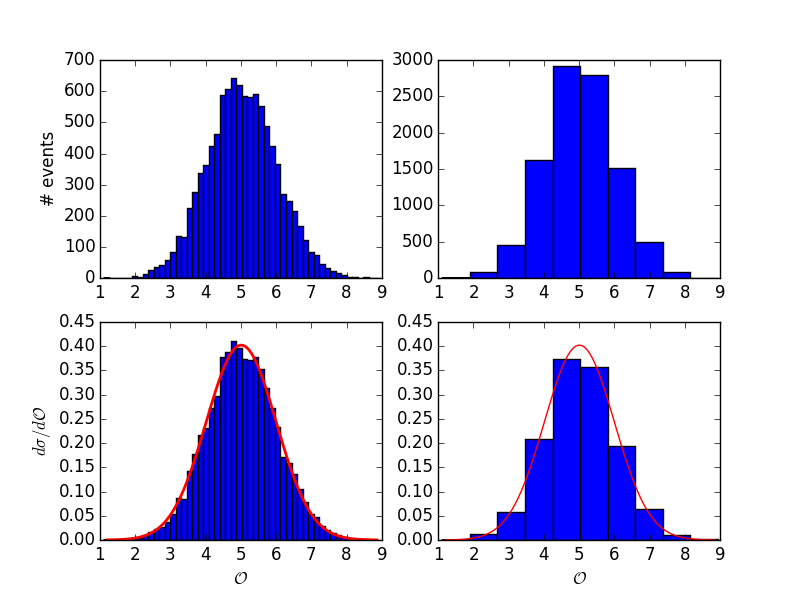
\includegraphics[scale=0.8]{images/histograms.png}  
\caption{The same data binned in two different ways, with two different binnings. }\label{fig:histograms}\end{figure}
%%\lecture{9}
\section{Calculating cross sections}
We can calculate cross sections using Fermi's second golden rule. It states that the transition rate per target particle and per beam particle $W$ is given by (see Bransden and Joachain, ch. 9)
\[\frac{\dot N}{N_a N_b}\equiv W=\frac{2\pi}{\hbar}\left|\mathcal{M}_{fi}\right|^2\rho(E')\]
where $\rho(E')$ is the density of final states. The transition matrix element $\mathcal{M}_{fi}$ between initial states $\psi_i$ and final state $\psi_f$ is given by:
\[\mathcal{M}_{fi}=\left<\psi_f|\mathcal{H}_{int}|\psi_i\right>\]
with $\mathcal{H}_{int}$ is the interaction Hamiltonian.
We can relate the transition rate to the cross section using eq.~\ref{eq:fluxa} and eq.~\ref{eq:ndot}
\[\dot N = n_a v_a N_b \sigma =\frac{N_a}{V} v_a N_b \sigma
\qquad
\Rightarrow
\qquad
W\equiv \frac{\dot N}{N_a N_b}=\frac{v_a\sigma}{V}
 \]
from which we get the cross section
\begin{equation}\label{eq:xsection}
\sigma=\frac{2\pi}{v_a}\left|\mathcal{M}_{fi}\right|^2\rho(E') V\;.\end{equation}
The volume dependence will cancel with the normalisation of the wave functions $\psi_i$ and $\psi_f$ entering the matrix element.
%
%
\subsection{Rutherford scattering}
%
%
%
We consider the scattering of a beam particle with energy $E$, momentum $p$ and  charge $ze$ off a charge distribution $\rho(x)$ of total charge $Ze$. We will consider the target to be much heavier than the probe, so that we can neglect the recoil and the outgoing energy of the scattered particle is the same as its incoming energy. We want to calculate the cross section in perturbation theory, so we need the interaction to be small which is the case if $Z\alpha\ll 1$. 
%%\keypoint{The Rutherford cross section describes the elastic scattering of a charged particle off the potential created by another charge.}
To calculate the cross section we need the transition matrix element
\[\mathcal{M}_{fi}=\left<\psi_f|\mathcal{H}_{int}|\psi_i\right>\;.\]
We describe the initial and final states as plane-waves
\[\psi_i=\frac{1}{\sqrt{V}}e^{i\V{p}\cdot\V{x}}\;,\qquad \psi_f=\frac{1}{\sqrt{V}}e^{i\V{p'}\cdot\V{x}}\]
where $\V{p}$ and $\V{p'}$ are the (three-)momenta of the incoming and outgoing particles. We chose the normalisation of the wave function such that there is one particle per volume $V$. The interaction Hamiltonian is given by the electromagnetic potential
\[\mathcal{H}_{int}(x)=ze\phi(x)\]


so that we get for the matrix element
\[\mathcal{M}_{fi}=\left<\psi_f|\mathcal{H}_{int}|\psi_i\right>
=ze\int dx\,\psi_f^*(x)\phi(x)\psi_i(x)\;.
=\frac{ze}{V}\int dx\,e^{-i\V{p'}\cdot x}\phi(x)e^{i\V{p}\cdot\V{x}}
=\frac{ze}{V}\int dx\,e^{i\V{q}\cdot x}\phi(x)\;.
\]
where we used the momentum transfer $\V{q}=\V{p}-\V{p'}$. There are different ways of proceeding from here, see ch. 5.2 of the book for a different way. To calculate the matrix element we first consider a simpler example where the charge distribution is point-like, and therefore the potential takes the usual $1/r$ form of the Coulomb potential. 
\[\rho(x)=Ze\delta^{3}(\V{x}-\V{x}_0)\;,\quad \phi(x)=\frac{Ze}{\left|\V{x}-\V{x}_0\right|}\] 
Inserting this in the matrix element calculation yields
\[\mathcal{M}_{fi}=\left<\psi_f|\mathcal{H}_{int}|\psi_i\right>
=\frac{ze}{V}\int d^3x\,e^{i\V{q}\cdot x}\phi(x)
=\frac{ze}{V}\int d^3x\,e^{i\V{q}\cdot x}\frac{Ze}{\left|\V{x}-\V{x}_0\right|}
\;.
\]
There is a small problem with this integral: it does not converge well. This is a reflection of the fact that the electromagnetic potential does not vanish quickly enough for the usual assumptions about the localisation of the potential to be fulfilled. The result is that the result of the integral will depend on the detail of the wave-functions at the boundary of the volume $V$. To avoid these complication many textbooks use an identity
\[\int\limits_V\left(u\bigtriangleup v-v\bigtriangleup u\right)\;dV = \oint\limits_{S} \left(v\nabla u - u\nabla v \right)\;dS\]
and argue that for a large enough volume the surface integral vanishes (but it does not, at least not for arbitrary volumes). Instead we are going to use a slightly modified potential that does vanish quickly enough for large volumes 
\[\phi(x)=\frac{Ze}{|\V{x}-\V{x_0}|}e^{-M |\V{x}-\V{x_0}|}\]
where the exponential factor ensures that our integrals converge. If we then take the limit $M\rightarrow 0$ we recover the pure Coulomb potential. 

To perform the integral we now change variable to $\V{x'}=\V{x}-\V{x}_0$ and introduce polar coordinates for the $\V{x}$ integration. We can choose the $z$ axis to be along the direction of $\V{q}$, so we get
\begin{eqnarray*}\label{eq:Mfi}
   \mathcal{M}_{fi}&=&
  \frac{ze}{V}\int d^3x\,e^{i\V{q}\cdot x}\frac{Ze}{\left|\V{x}-\V{x}_0\right|}e^{-M\left|\V{x}-\V{x}_0\right|}
  =
  \frac{e^2zZ}{V}\int d^3x'\,e^{i\V{q}\cdot \V{x_0}}\,e^{i\V{q}\cdot \V{x'}-M|\V{x'}|}\frac{1}{\left|\V{x'}\right|}\\
  &=&
  \frac{e^2zZ}{V}e^{i\V{q}\cdot \V{x_0}}2\pi\int\limits_0^\infty r^2\, dr\int\limits_{-1}^{1}d\cos\theta \,e^{i|\V{q}|r\cos\theta-Mr}\,\frac{1}{r}
  =
  \frac{2\pi e^2zZ}{V}e^{i\V{q}\cdot \V{x_0}}\int\limits_0^\infty r\, dr\left. \frac{1}{i|\V{q}|r}e^{i|\V{q}|r\cos\theta-Mr}\right|_{\cos\theta=-1}^{\cos\theta=+1}\\
  &=&\frac{2\pi e^2zZ}{V}e^{i\V{q}\cdot \V{x_0}}\int\limits_0^\infty \, dr\frac{1}{i|\V{q}|}\left(e^{i|\V{q}|r-Mr}-e^{-i|\V{q}|r-Mr}\right)
  =
  \frac{2\pi e^2zZ}{i|\V{q}|V}e^{i\V{q}\cdot \V{x_0}} \left. \left(\frac{e^{i|\V{q}|r-Mr}}{i|\V{q}|-M}-\frac{e^{-i|\V{q}|r-Mr}}{-i|\V{q}|-M}\right)\right|_0^\infty
  \\
  &=&
  \frac{2\pi e^2zZ}{i|\V{q}|V}e^{i\V{q}\cdot \V{x_0}}  \left(-\frac{1}{i|\V{q}|-M}+\frac{1}{-i|\V{q}|-M}\right)
  =
    \frac{2\pi e^2zZ}{i|\V{q}|V}e^{i\V{q}\cdot \V{x_0}}  \frac{i|\V{q}|+M+i|\V{q}|-M}{|\V{q}|^2+M^2}
\\    &=&
    \frac{4\pi e^2zZ}{V}e^{i\V{q}\cdot \V{x_0}}  \frac{1}{|\V{q}|^2+M^2}
\end{eqnarray*}

  

\begin{wrapfigure}{r}{0.5\textwidth}
	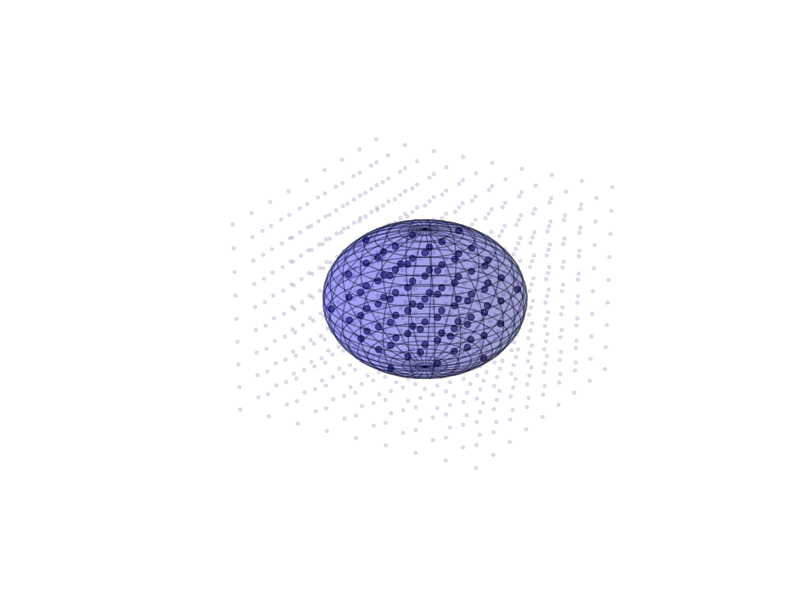
\includegraphics[scale=0.7,trim=5cm 5cm 5cm 5cm,clip=true]{images/PSsphere.png}
 \caption{Illustration for the number of states in a box volume. Only momenta with components $p_i=n 2\pi/L$ are allowed (represented by dots in the figure.) The number of states is the number of dots inside the sphere (shown in black in the figure.) }\label{fig:densityOfStates}
\end{wrapfigure}

Taking the limit $M\rightarrow 0$ we get the result quoted in the book
\[\mathcal{M}_{fi}= \frac{4\pi e^2zZ}{V}e^{i\V{q}\cdot \V{x_0}}  \frac{1}{|\V{q}|^2} \]

The last ingredient we need is the density of final states. In our case the final states can be labelled by their momenta $\V{p}'$. Imposing boundary conditions for the wave functions at the boundary of the volume $V$ restricts the number of possible values of $\V{p}'$. If we take the volume to be a cube of length $L$ and impose periodic boundary conditions for the plane wave $e^{i\V{x}\cdot\V{p}}$ we get the condition $p_i L=2\pi n$ with $n$ an integer. So values of $\V{p}'$ are placed on at three-dimensional lattice with spacing $2\pi/L$. To obtain the number of states in a volume of values on $\V{p'}$ one needs to divide this volume by $(2\pi/L)^3=(2\pi)^3/V$. 

The final state volume is given by
\[\int d^3\V{p}=\int d\Omega |\V{p'}|^2\,d|\V{p'}|\] 
so that the number of final states is given by
\[ dn(|\V{p'}|)=\frac{V}{(2\pi)^3} d\Omega |\V{p'}|^2\,d|\V{p'}|\]
For the golden rule we need the density of states $dn/dE'$:
\begin{equation}\label{eq:Edensity}
d\rho(E')=\frac{dn}{dE'}=\frac{V}{(2\pi)^3} d\Omega |\V{p'}|^2\frac{d|\V{p'}|}{dE'}= \frac{V}{(2\pi)^3} d\Omega |\V{p'}|^2 
\end{equation}
where the high energy limit $|p'|\simeq E'$ was used.

Putting the matrix element eq.~(\ref{eq:Mfi}), the final state density eq.~(\ref{eq:Edensity}) in the cross section formula eq.~(\ref{eq:xsection}) we get
\begin{eqnarray*}
d	\sigma&=&\frac{2\pi}{v_a}\left|\mathcal{M}_{fi}\right|^2\,V\,d\rho(E')  \nonumber\\
&=& \frac{2\pi}{v_a} \left|\frac{4\pi e^2zZ}{V}e^{i\V{q}\cdot \V{x_0}}  \frac{1}{|\V{q	}|^2}\right|^2\,V\,\frac{V}{(2\pi)^3} d\Omega |\V{p'}|^2 
\nonumber\\
&=&\frac{4e^4z^2Z^2}{|\V{q}|^4} d\Omega E'^2 
\end{eqnarray*}
where we have assumed that the speed $v_a$ was the speed of light. We get the differential cross section:
\begin{equation}
\frac{d\sigma}{d\Omega}=\frac{4e^4z^2Z^2 \,E'^2}{|\V{q}|^4}  \;.
\end{equation}
We can express this cross section as a function of the scattering angle $\theta$, using the fact that $\V{q}=\V{p}-\V{p'}$.
%%\image{ppprimeq.png}
\begin{figure}
\begin{center}
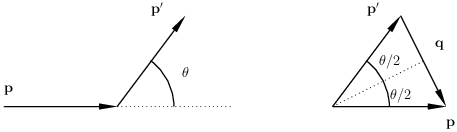
\includegraphics[scale=0.45]{images/ppprimeq.png}
\end{center}
\caption{Scattering kinematics.}\label{fig:rutherfordKin}
\end{figure}
\[|\V{q}|=2 |\V{p}|\sin\frac{\theta}{2}\;,\qquad \frac{d\sigma}{d\Omega}=\frac{e^4z^2Z^2 \,E'^2}{4|\V{p}|^4\sin^4\frac{\theta}{2}}= \frac{e^4z^2Z^2}{4E^2\sin^4\frac{\theta}{2}}\;, \]
where we have used the assumption the the scattering is elastic $E=E'$ and used the high energy limit $|\V{p}|=E$. This is the Rutherford scattering formula.
\pagebreak 
%
%
%%\lecture{10}
%%\section{The Mott Cross Section}
\section{Mott cross section}


\begin{wrapfigure}{r}{0.4\textwidth}
\begin{center}
%%\image{rutherfordMott.png}
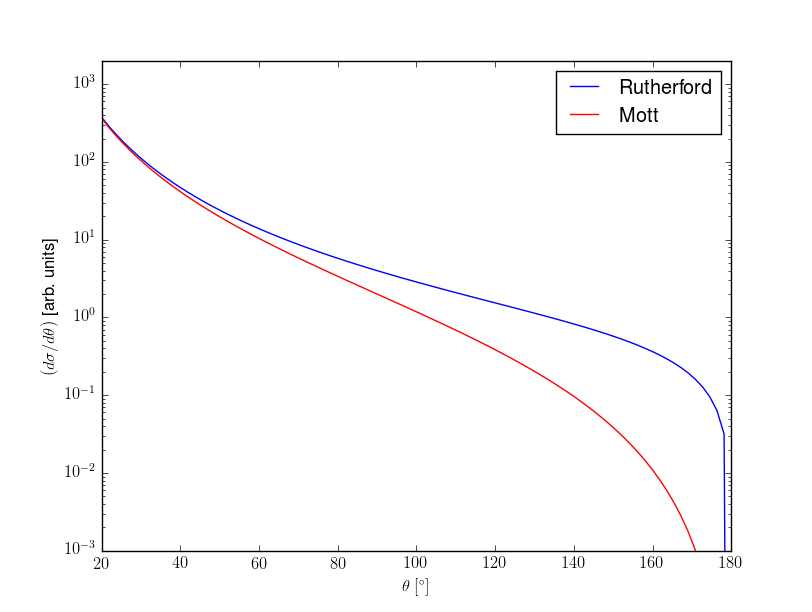
\includegraphics[scale=0.35]{images/rutherfordMott.png}
\end{center}
\caption{Rutherford and Mott differential cross sections as a function of the scattering angle. The Mott cross section is suppressed at large angles compared with the Rutherford cross section.}\label{fig:mottVSruth}
\end{wrapfigure}
So far we have neglected the spin effects. If we include the effect of the spin of the electron (but still neglect the nucleus recoil) we get the Mott cross section 
%%\keypoint{ When the projectile is relativistic, its spin has to be taken into account, this leads to the Mott cross section.}
\begin{equation}\label{eq:Mott}
\left(\frac{d\sigma}{d\Omega}\right)_{\rm{Mott,no\; recoil}}=\left(\frac{d\sigma}{d\Omega}\right)_{\rm{Rutherford}}\left(1-\beta^2\sin^2\frac{\theta}{2}\right)
\end{equation}
where $\beta=v/c$ with $v$ the velocity of the electron. In the high energy limit $\beta\simeq 1$ so that we get
\[\left(\frac{d\sigma}{d\Omega}\right)_{\rm{Mott,no\; recoil}}=\left(\frac{d\sigma}{d\Omega}\right)_{\rm{Rutherford}}\cos^2\frac{\theta}{2}\]
The spin effect is to reduce the cross section as the scattering angle increases. In the extreme case of backward scattering $\theta=180^\circ$ the differential cross section vanishes. The reason for this effect is that for relativistic spin $1/2$ fermions with $\beta=1$ the spin measured in the direction of motion is conserved, in other words the helicity $h$
\[h=\frac{\V{s}\cdot\V{p}}{|\V{s}||\V{p}|}\]
cannot change. In the case of backward scattering if the spin of the incoming particle was aligned with its direction (say along the $z$-axis) after scattering it would have to be pointing along the opposite direction, since this is the direction of the recoiled electron and helicity is conserved. But in this case angular momentum would not be conserved! If the angle is not $180^\circ$ then there is an overlap between the wave function of the incoming and outgoing electrons with spins aligned with their momenta. This overlap increases as the directions of the incoming and outgoing particles get more and more aligned.
%%\keypoint{Helicity conservation suppresses backward scattering.}
\begin{figure}
\begin{center}
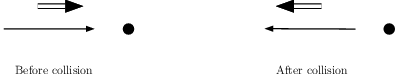
\includegraphics[scale=0.7]{images/scattering180.png}
\caption{180 degrees scattering.}\label{fig:180deg}
\end{center}
\end{figure}
%
%
%
%
%
%%\section{Nuclear Form Factors}
\section{Nuclear form factors}
So far we have only considered point-like potentials. To obtain the matrix element for an extended charge distribution $\rho(x)=Ze\,f(x)$ with the normalisation $\int f(x)\,dx=1$ we can use 
\[\rho(x)=\int \rho(y)\delta(x-y)\,dy=Ze\int f(y)\delta(x-y)\,dy\quad\Rightarrow \quad \phi(x)=Ze\int f(y)\frac{1}{|x-y|}\,dy \] 
to obtain 
\begin{eqnarray}
\mathcal{M}_{fi}&=&\left<\psi_f|\mathcal{H}_{int}|\psi_i\right>
=\frac{e}{V}\int d^3x\,e^{i\V{q}\cdot x}\phi(x)\nonumber\\
&=&
\frac{e}{V}\int d^3x\,e^{i\V{q}\cdot x}Ze\,\int f(y)\frac{1}{\left|\V{x}-\V{y}\right|}\,d^3y
=
\frac{Ze^2}{V}\int \,d^3y\,f(y)\int d^3x\,e^{i\V{q}\cdot x}\frac{1}{\left|\V{x}-\V{y}\right|}\nonumber\\
&=&
\frac{Ze^2}{V}\int \,d^3y\,f(y)\frac{4\pi}{|\V{q}^2|}\,e^{i\V{q}\cdot y}
=
\frac{4 \pi Z e^2}{V|\V{q}^2|}\int \,d^3y\,f(y)\,e^{i\V{q}\cdot y}\nonumber\\
&\equiv&\frac{4 \pi Ze^2}{V|\V{q}^2|}F(q)
\end{eqnarray}
where \[
F(q)=\int \,d^3y\,f(y)\,e^{i\V{q}\cdot y}
\] is called the form factor. If the distribution is point-like the form factor is $F(q)=1$ and we recover the previous result. If the charge distribution is not point-like, then the form factor will be reduced from its value of $1$ as the value of $|\V{q}|$ is such that $1/|\V{q}|$ is of the order of the spacial extent of the charge distribution. 
%%\keypoint{If the scattering is off a charge distribution instead of a point-particle then the matrix element is reduced by a factor called the form factor. The form factor is the Fourier transform of the charge distribution. The cross section is reduced by the square of the magnitude of the form factor.}

A similar reasoning can be applied if we want to take the spin effect of the electron into account and we get:
\[\left(\frac{d\sigma}{d\Omega}\right)_{\rho(x)}=\left(\frac{d\sigma}{d\Omega}\right)_{\rm{Mott,no\; recoil}}\left|F(\V{q})\right|^2\]   
This offers the possibility to investigate the charge distribution by looking at the ratio between the Mott cross section and the measured cross section. These two cross sections are plotted in fig.~\ref{fig:CaXsection}. 
 
\begin{figure}
%%\image{CaFormFactor.png}
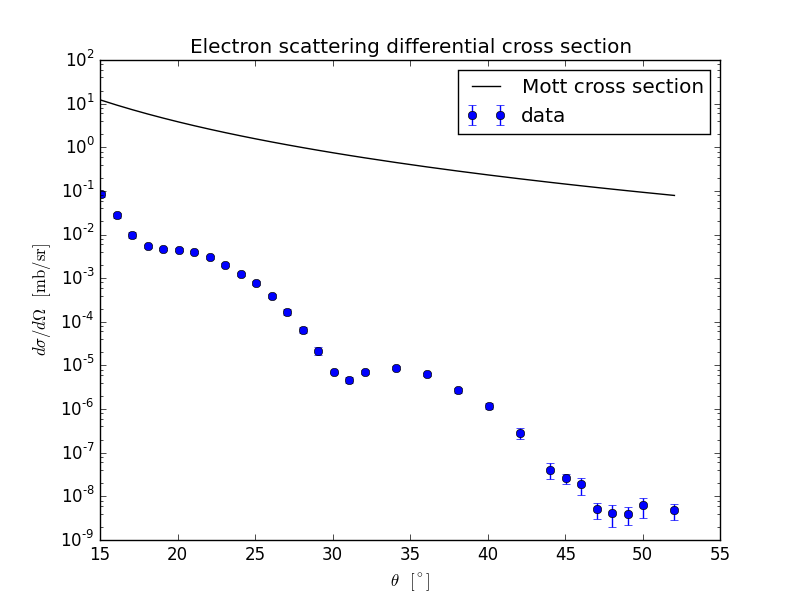
\includegraphics[scale=0.4]{images/CaXsection.png}
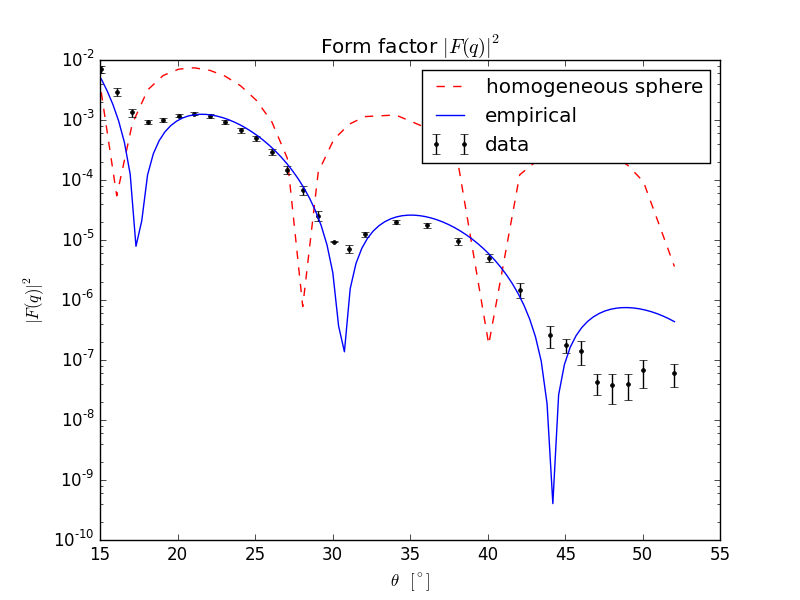
\includegraphics[scale=0.4]{images/CaFormFactor.png}
\caption{The left panel shows the measured cross section and Mott cross section for the scattering of an electron of energy $757.5\,\rm{MeV}$ off a calcium nucleus. The right-hand side panel shows the ratio of the two cross sections which is the form factor and the prediction using two different model: an homogeneous sphere of radius $4.13\;\rm{fm}$ and a charge distribution based on eq.~\ref{eq:fermi} with $r_0=3.66\;\rm{fm}$ and $a=0.54\;\rm{fm}$.}\label{fig:CaXsection}
\end{figure}

By taking the ratio we get the square of the form factor $F(\V(q))$. If the charge distribution $f(\V{x})$ is spherically symmetric ($f(\V{x})=f(|\V{x}|)$)the form factor can be written as
\[F(\V{q})=\int e^{i\V{q}\cdot\V{x}}f(\V{x})\,d^3x=4\pi\int f(r)\frac{\sin |\V{q}| r}{|\V{q}| r}r^2\,dr\]
in this case the form factor only depends on the length of $\V{q}$ so it is often written as $F(q^2)$. Different charge distributions lead to different functional dependencies.
\begin{figure}
\begin{center}
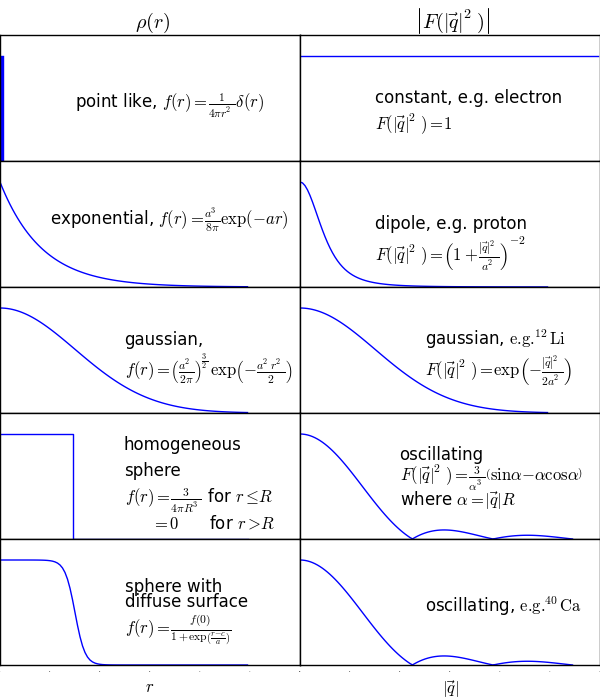
\includegraphics[scale=0.9]{images/form.png}
\end{center}
\caption{Form factor for several charge distributions}\label{fig:formFactor}
\end{figure} 
For example the form factor for an homogeneous sphere of radius $R$ is given by
\[F(q^2)=\frac{3}{a^3}\left(\sin a-a\cos a\right)\;,\quad\mbox{with}\quad a=|\V{q}|R\]
the term in parenthesis has zeros for several values of $a$:
\[\left(\sin a-a\cos a\right)=0\;\Rightarrow\;a\simeq 4.49341,7.72525,10.9041,14.0662,17.2208,\dots\]
So if we assume this charge distribution and we can locate the first minimum of the form factor $q_0$ we can infer the radius of the sphere:
\[a_0=|q_0|R\simeq 4.49341\;\Rightarrow R\simeq\frac{4.49341}{q_0}\;.\] 
In practice it is found experimentally that the charge distribution are not homogeneous but can be described quite well using a two-parameter Fermi function as an approximation of the charge distribution: 
\begin{equation}\label{eq:fermi}
f(r)=\frac{f_0}{1+e^{\frac{r-r_0}{a}}}
\end{equation}
where $f_0$ is chosen such that 
\[4\pi\int dr \,r^2 f(r)=1\;.\]
Figure~\ref{fig:chargeDistribution} shows the experimentally measured charge distribution\footnote{Nuclear Physics A, Volume 235, Issue 1, Pages 1-266 (9 December 1974), B. Dreher, J. Friedrich, K. Merle, H. Rothhaas, G. Lührs, Pages 219-248} and the approximation based on the above formula. 
\begin{figure}
%%\image{ChargeDistribution.png}
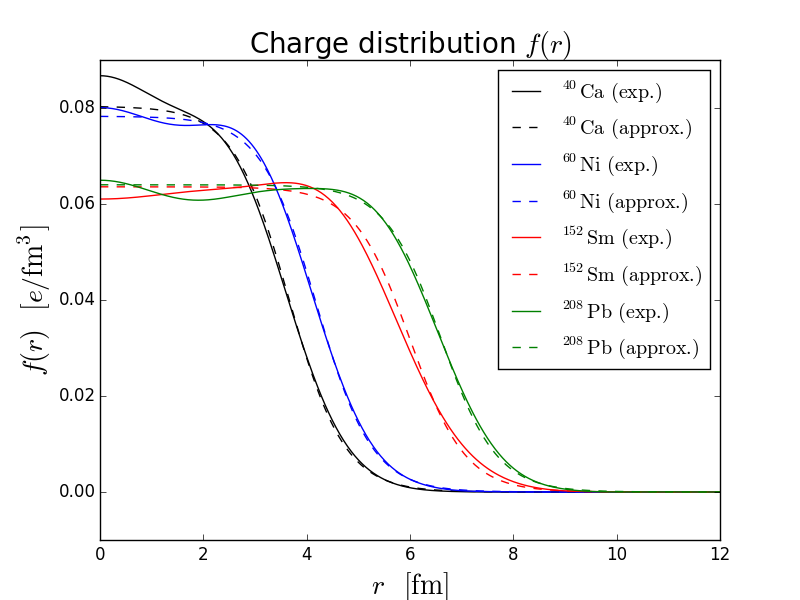
\includegraphics[scale=0.6]{images/ChargeDistribution.png}
\caption{Experimental charge distribution for four nuclei and the approximation based on eq.~(\ref{eq:fermi}). }\label{fig:chargeDistribution}
\end{figure}
%%\keypoint{Looking at the ratio between the point-like cross section and the actual cross section one can infer the form of the charge distribution. Using this technique one can measure the charge distribution in the nucleus of an atom.}
%
%
%
%
%%\lecture{11}
%%\section{Scattering off Nucleons}
\section{Scattering off nucleons}
%%\keypoint{One can use the form factor technique to measure the charge distribution of the proton or neutron. In this case we need to consider the magnetic interaction due to the spin of the nucleon and one can measure both the electric charge and the magnetic moment distribution inside the nucleons.}
We have seen elastic scattering off nuclei, we would now like to concentrate on the properties of the components of the nucleus: the proton and neutrons. Given that their size is of the order of  $1\rm{fm}$ we need electrons with energy $q=1/1\rm{fm}\simeq 200\,\rm{MeV}$ which is not negligible compared with the nucleon mass $M\simeq 938\,\rm{MeV}$. Luckily the changes for the Mott cross section are not big: a) one needs to replace the momentum transfer $\vec{q}$ with a Lorentz invariant quantity $q$:
\[\V{q}\rightarrow q=p-p'=(E-E',\V{p}-\V{p'})\;,\quad \V{q}^2\rightarrow -q^2=-(E-E')^2+(\V{p}-\V{p'})^2\equiv Q^2\] 
since the invariant mass $q^2$ of $q$ is negative we use $Q^2=-q^2$ so that we have a positive quantity. b) one needs to multiply the cross section with $E'/E$, this is due to the fact that the density of final states must now take the momentum of the recoiling nucleon into account. So the cross section taking the recoil into account is given in the high energy limit by
\[
\left.\frac{d\sigma}{d\Omega}\right|_{\rm{with}\;\rm{recoil}}
=
\frac{\alpha^2}{4E^2\sin^4\frac{\theta}{2}}
\left(
\frac{E'}{E}\right)
\left[
\cos^2\frac{\theta}{2}+\frac{Q^2}{2M^2}\sin^2\frac{\theta}{2}\right]
=
\left.\frac{d\sigma}{d\Omega}\right|_{\rm{Mott}} \left[
1+2\tau\tan^2\frac{\theta}{2}\right]\;.
\]	
with 
\[\tau=\frac{Q^2}{4M^2}\]
The term proportional to $\tan^2\theta/2$ is caused by the magnetic interaction of the electron current with the magnetic moment of the nucleon, which is given by 
\[\mu=g\frac{e}{2M}\frac{1}{2}\]
with $g=2$ for a spin $1/2$ fermion (it is a consequence of the Dirac equation). The interaction through this term is accompanied by a flip of the  
spin of the nucleon, so we have the opposite situation as earlier where angular momentum restricted the large angle scattering. 
\begin{figure}
\begin{center}
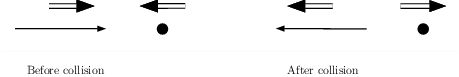
\includegraphics[scale=0.7]{images/scattering180b.png}
\end{center}
\caption{When a spin flip of the nucleon is allowed the large angle scattering is allowed and the small angle one is forbidden.}\label{fig:spinflip}
\end{figure}
This formula is valid for the nucleon when treated as a point-like object. Since we want to investigate the structure of the nucleon we will make the same step as when we investigated the charge distribution inside a nucleus. Calculating the cross section for an object with a finite size will modify the cross section in the same way as before: it will be multiplied by the square of the Fourier transform of the distribution. This time both the electric and magnetic interaction are important, so we will need both the Fourier transform of the charge distribution and that of the magnetic moment.

The result is called the Rosenbluth formula. It describes the relativistic scattering of an electron off a target with a spatial electric charge density and a spatial magnetic moment density.
\[\frac{d\sigma}{d\Omega}=\left(\frac{d\sigma}{d\Omega}\right)_{\rm  Mott} \left[\frac{G^2_E(Q^2)+\tau G^2_M(Q^2)}{1+\tau}+2\tau G^2_M(Q^2)\tan^2\frac{\theta}{2}\right]\;,\quad \tau=\frac{Q^2}{4M^2_p}\;,\]
we now have two form factors, $G_E(Q^2)$ is related to the Fourier transform of the electric charge density, while $G_M(Q^2)$ is the form factor associated with the magnetic moment density. The derivation of this formula is beyond the remit of the course. If we set the magnetic form factor to $0$ we recover the formula for the scattering off an electric charge density (with relativistic factors now). We also see that the angular dependence (beyond the kinematical one brought by $1/q^4$) comes only with the magnetic form factor $G_M(Q^2)$.

If the nucleons were point-like we would find that the form factors $G_E(Q^2)$ and $G_M(Q^2)$ would be constant. Since they are not, we will observe the same fall-off at values of $Q^2$ of the order of the inverse spacial extend of the probe $Q\simeq 1/R$. One way of seeing this effect is that when $Q^2$ is very large the scattering particle only interacts with a small part of the probe, for example with a small portion of the charge and hence the cross section is diminished.

For small values of $Q^2\ll 1/R^2$ the nucleon appears to be a point-like particle and we should recover the point-like result. We find for the proton:
\[G_E^p(Q^2=0)=1\;,\quad G_M^p(Q^2=0)=2.79\]
the first value is as expected the charge of the proton, but the value of $G_M$ would be $1$ for a Dirac particle of spin $1/2$. The fact that it is not the case is due to the fact that the proton has an internal structure and its response to a magnetic field is not as simple as that of a structure-less Dirac particle. For the neutron we find:
\[G_E^p(Q^2=0)=0\;,\quad G_M^p(Q^2=0)=-1.91\;,\] 
where again the electric form factor $G_E$ tends for low $Q^2$ towards the charge of the nucleon, and the magnetic moment shows that the neutron has an internal structure. 

\begin{wrapfigure}{r}{0.6\textwidth}
\begin{center}
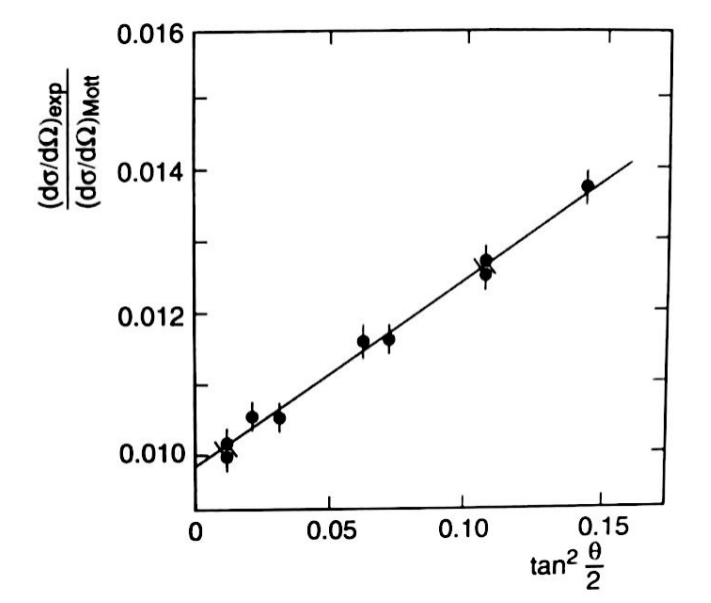
\includegraphics[scale=0.35,trim=1cm 0.5cm 0.5cm 0.7cm,clip=true]{images/FormFactorOfTan.png}
\end{center}
\caption{Ratio of the experimental and Mott cross section for a fixed momentum transfer $Q^2=2.5 {\rm GeV^2}$. Data from \cite{Taylor}, figure from \cite{povh}. }\label{fig:mottfixedQ}
\end{wrapfigure}
The form factors are measured for a fixed value of $Q^2$ by looking at the $\theta$ dependence of the ratio
\[\frac{
\left(\frac{d\sigma}{d\Omega}\right)_{\rm exp}
}{
\left(\frac{d\sigma}{d\Omega}\right)_{\rm  Mott}
}
\]
and fitting the coefficients $G_E(Q^2)$ and $G_M(Q^2)$. This is illustrated in the figure on the right: The intersection of the fit with the $y$-axis corresponds to 
\[\frac{G^2_E(Q^2)+\tau G^2_M(Q^2)}{1+\tau}\]
and the slope is 
\[2\tau G^2_M(Q^2)\;.\]
We can now plot the values of the form factors $G_E(Q^2)$ and $G_M(Q^2)$. An example of the $Q^2$ dependence of the form factors is shown in Figure~\ref{fig:FormFactorOfQ2}. 
\begin{figure}
\begin{center}
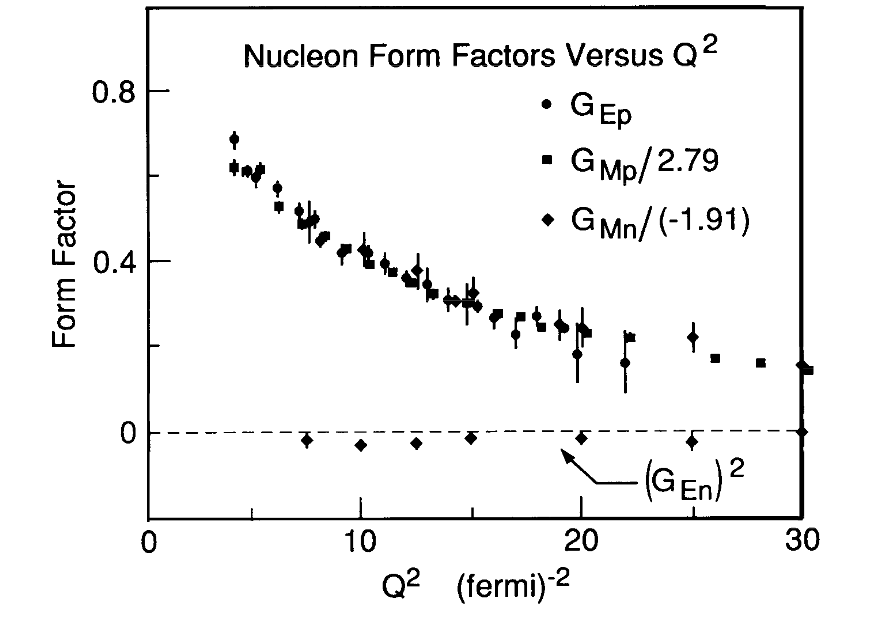
\includegraphics[scale=0.4]{images/FormFactorOfQ2.png}
\end{center}
\caption{Electric and magnetic form factors for the proton and neutron as a function of the momentum transfer $Q^2$. Data from \cite{Hughes:1966zz}}\label{fig:FormFactorOfQ2}
\end{figure}
We can see in this Figure that the form factor is not constant and has a dependence on $Q^2$. The dependence on $Q^2$ can be used to infer the distribution of charge and magnetic moment in the nucleon. For the proton electric form factor and the magnetic form factor of both nucleon the $Q^2$ dependence can be described well by a dipole form
\[G(q^2)\simeq\frac{1}{1+q^2/a^2}\;.\]
Looking at Figure~\ref{fig:formFactor} we can infer that the charge and magnetic moments are distributed according to and exponentially falling distribution. It is also noteworthy that the electric form factor of the neutron is not completely vanishing, as one would expect if there were no charge in the neutron. We will see later that the neutron is composed of quarks which carry charges and their spatial charge distribution is not completely vanishing but cancel exactly when integrated over the neutron volume. 

\section{From Quantum Mechanics to Quantum Field Theory}
So far we have considered the scattering problem in a quantum mechanical way. We have computed the overlap between initial and final state wave functions given an interaction potential. This description only works for the simplest problems. To describe particle physics accurately we need to overcome a serious limitation of the QM description, namely that the number of particle is conserved. 

In a typical particle collision some particle annihilate and new particles are created so we need to be able to create new states instead of just observing the evolution of a given state to another one. Quantum field theory is an appropriate description for particle collisions where new particles are created but it is beyond the remit of this course. In this section we describe some of the implications of QFT. 

\begin{figure}
\begin{center}
%%\image{QFT.png}
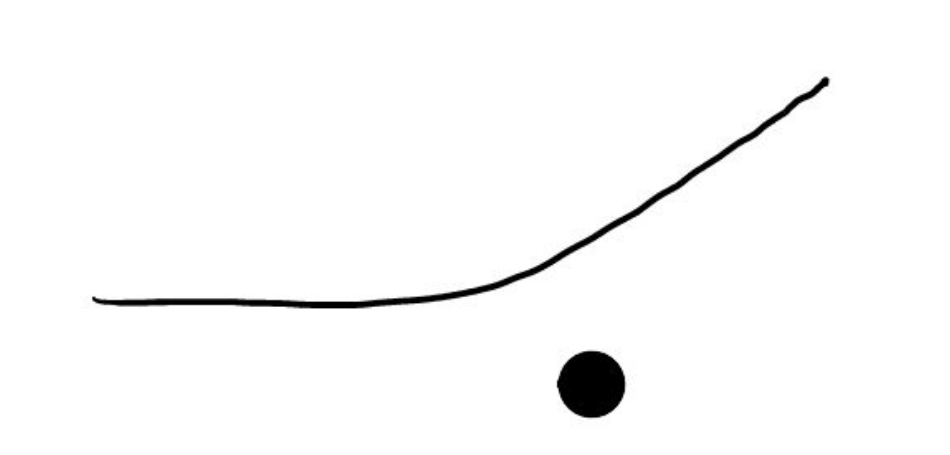
\includegraphics[scale=0.2]{images/QM.png}  
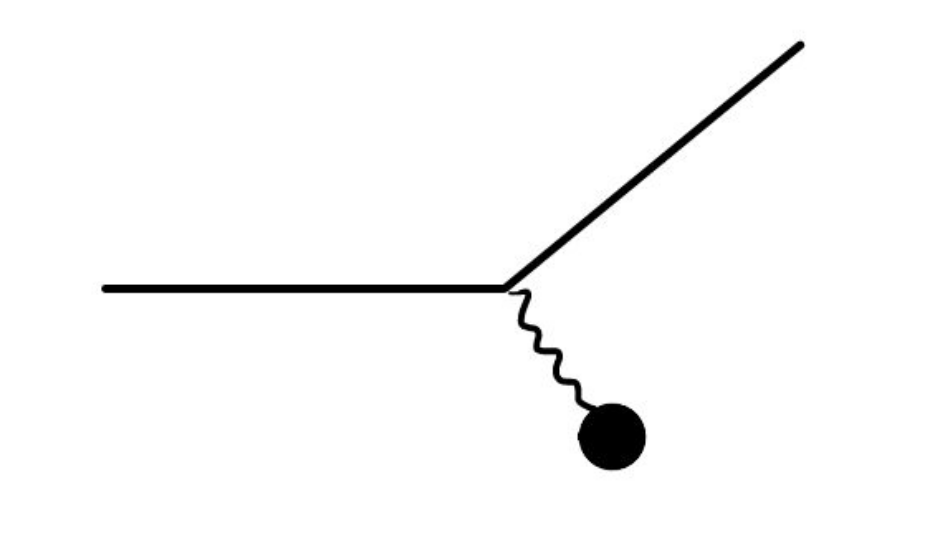
\includegraphics[scale=0.2]{images/QFT.png}  
\end{center}
\caption{The left-hand panel illustrates the scattering off a potential. The right-hand side illustrate the scattering as describe in QFT where the interaction is "quantised" and mediated through a virtual particle.}\label{fig:QMvsQFT}
\end{figure}

In Quantum mechanics the interaction is described by a potential that acts "continuously" on the state. In QFT the interaction is "quantised" and the action of the force is mediated by particles. In the example of the electro-magnetic force the mediator is the photon. 

\begin{wrapfigure}{r}{0.5\textwidth}
\begin{center}
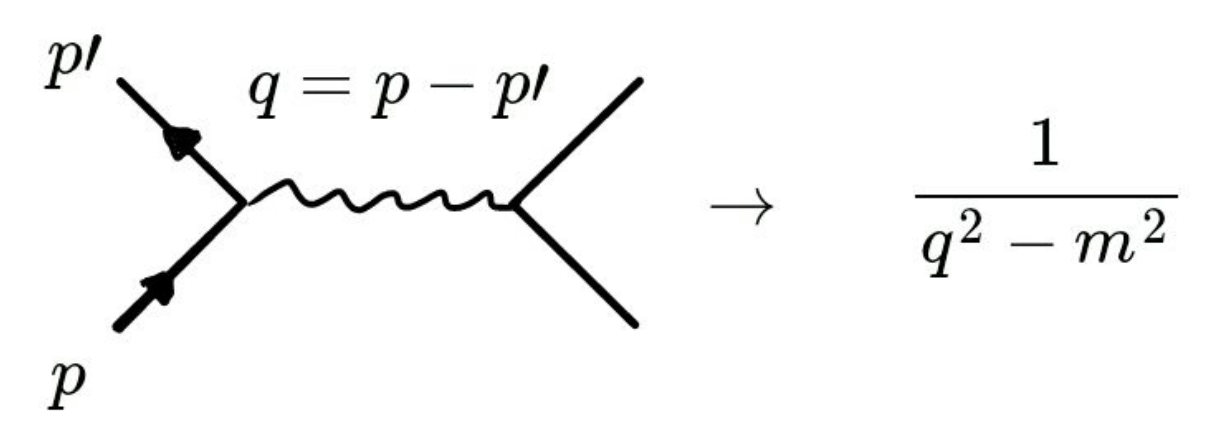
\includegraphics[scale=0.2]{images/propagator.png}
\end{center}
\caption{A virtual particle leads to a factor in the amplitude inverse proportional to the distance of the squared four momentum to its "true" mass.}\label{fig:propagator}
\end{wrapfigure}
The particle exchange is a quantum mechanical effect and cannot be observed directly, only its effect is visible through the momentum that is transferred. Because it is not detectable the particle exchanged is called $virtual$. 

As they are not observed virtual particles can violate the relationship $p^2=m^2$ between their four-momentum and their mass. According to the uncertainty principle such a violation of the energy relation can only last for a time inverse proportional to the size of the energy difference. 

In general a process involving a virtual particle will have a factor in its amplitude inverse proportional to the violation of then mass relation. 
\begin{equation}\label{eq:propagator}
\mathcal{M}\simeq \frac{1}{q^2-m^2}
\end{equation}
where $q$ is the momentum carried by the particle and $m$ its rest mass. Such a factor is referred to as \emph{propagator}. We can now provide a more intuitive interpretation of the $Q^2$ dependence of the Rutherford scattering: the incoming electron emits a virtual photon with de Broglie wavelength proportional to $1/Q$. It is this wavelength that is relevant to fix the resolution of the scattering, and not the wavelength of the incoming electron. The $1/Q^4$ dependence of the Rutherford scattering is also explained by the form of the propagator \ref{eq:propagator} where the mass of the photon is $m=0$. 
\[\sigma\simeq |\mathcal{M}|^2\simeq \left(\frac{1}{q^2-0}\right)^2=\frac{1}{Q^4}\;.\]
%%\keypoint{If the energy of the scattering is large enough to be able to create and destroy states we need to go from Quantum Mechanics to Quantum Field Theory. One consequence is that forces are now mediated through the exchange of a particle.}
%
%
%%\lecture{12}
%%\section{Inelastic Scattering}
\section{Inelastic scattering}
\subsection{Nucleon excited states}
So far the scattering has always been elastic: the object off which we scatter is left unchanged (albeit with some recoil momentum). The next step we reach when increasing the energy of the scattering is that the target is now altered by the scattering: the scattering is inelastic. 
%%\keypoint{If the energy is further increased much above the proton mass the proton is changed after the scattering and the scattering is therefore non-elastic. As a consequence we now need two parameter to describe the scattering.}
The invariant mass of the target after the scattering $W^2$ is given by
\begin{eqnarray}\label{eq:FSinvariantMass}
W^2&=&\left(P+p-p'\right)^2=\left(P+q\right)^2=P^2+2P\cdot q-Q^2
\\
&=&M^2+2 P\cdot q -Q^2=M^2+2M\nu -Q^2
\end{eqnarray}
where $M$ is the mass of the proton and we have defined a new quantity
\begin{equation}\label{eq:DISnu}
\nu=\frac{P\cdot q}{M}\;.
\end{equation}
In the laboratory frame $\nu$ is the energy transfer:
\[\nu=\frac{P\cdot q}{M}=\frac{(M,0,0,0)\cdot(E-E',\vec p -\vec p')}{M}=\frac{M(E-E')}{M}=E-E'\;.\]
For elastic scattering, for which $W^2=M^2$ eq.~\ref{eq:FSinvariantMass} implies
\[2M\nu-Q^2=0\]
if the collision is inelastic, that is $W^2>M^2$ we have
\begin{equation}\label{eq:xInequality}
2M\nu-Q^2>0
\end{equation}
In elastic scattering we only had one parameter to describe the scattering, it could be chose to be $\theta$ the scattering angle or $Q^2$ the momentum transfer. Now in inelastic scattering we have two parameters, common choices are $E',\theta$ or $Q^2,\nu$.
%
\begin{figure}[h]
\begin{center}
%%\image{inelasticScatteringeP.png}
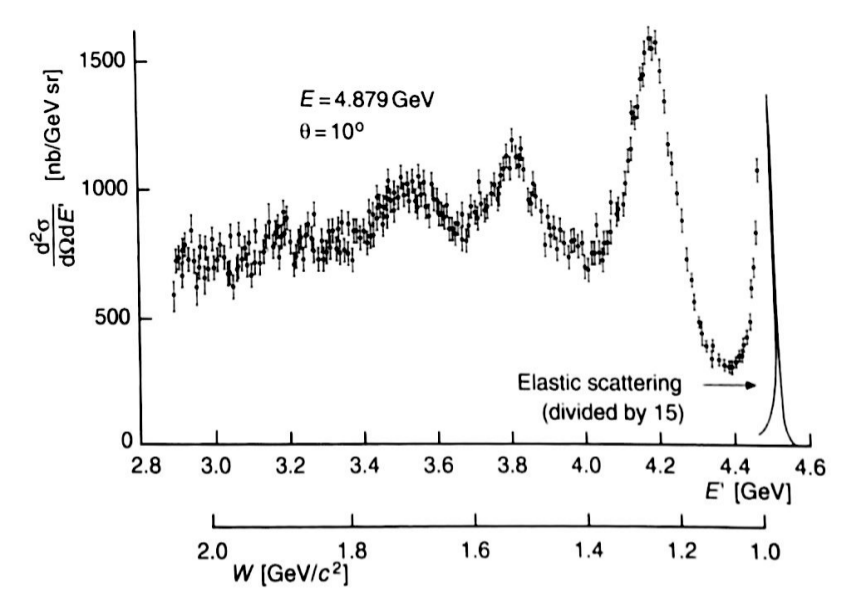
\includegraphics[scale=0.5]{images/inelasticScatteringeP.png}
\end{center}
\caption{Differential cross section for an electron off a proton for a fixed scattering angle of $10^o$ and a beam energy of $4.9\,\mbox{GeV}$. Data from \cite{Bartel:1968tw} and figure from \cite{povh}.}\label{fig:DISspectrum}
\end{figure}
%
Figure \ref{fig:DISspectrum} shows the differential cross section as a function of $E'$ for a fixed value of $\theta$. The second $x$ axis is shows the corresponding values of $W^2$. At the right of the plot we have the elastic scattering peak, to fit in the figure its height has been reduced by a factor of 15. When we were considering elastic scattering this is the only events we were considering and the value of $E'$ was fixed to its maximum value (and $W^2$ was fixed to $M^2$.) The peak at $W\simeq 1.25\,\mbox{GeV}$ is caused by the $\Delta^+$ resonance (we will learn more about it later), the peaks further to the left are higher resonances.  

%
%
%%\section{Deep Inelastic Scattering}
 \subsection{Deep inelastic scattering}
%
%
%

We can follow the same strategy as we did so far: formulating the most general form the scattering can take and introducing form factors for the parts that are dependent on the target composition. For inelastic scattering of an electron off a proton we use:
\[\frac{d\sigma}{d\Omega\,dE'}= \left(\frac{d\sigma}{d\Omega}\right)_{\rm  Mott, no\; recoil}\left[W_2(Q^2,\nu)+2W_1(Q^2,\nu)\tan^2\frac{\theta}{2}\right]   \]
where $W_1$ and $W_2$ are the ``form factors'' for the inelastic scattering, they are called structure functions. The parametric form of the cross section is due to the fact that the interaction is carried by a photon, but its derivation is again beyond the scope of this course. It is important to note that now the structure functions depend on two parameters, unlike in the case of elastic scattering. 
%%\keypoint{In a deep inelastic experiment one collides a large energy electron with a proton.}

It is useful to introduce a new quantity
\[x=\frac{Q^2}{2M\nu}\;.\]
Because we have seen in eq.~\ref{eq:xInequality} that $2M\nu -Q^2\geq 0$, with the equality holding for the case of elastic scattering we can conclude that
\[0<x\leq 1\]
where $x=1$ is the case for elastic scattering. This variable has the advantage to be dimensionless and we will see that $x$ take on a particular meaning in the parton model.
 
It is useful to express the structure functions $W_1$ and $W_2$ in terms of  dimensionless ones and to use $x$ instead of $\nu$ as the second free parameter in the structure constants:
\[F_1(x,Q^2)=MW_1(Q^2,\nu)\;,\quad F_2(x,Q^2)=\nu W_2(Q^2,\nu)\;.\]
The scattering cross section now takes the form
\begin{equation}\label{eq:diffCrossSectionStructureFunction}
\frac{{\rm d}^2\sigma}{{\rm d}x{\rm d}Q^2}
 = \frac{4\pi\alpha^2}{Q^4}\left[\left(1-y-\frac{M^2x^2y^2}{Q^2}\right)\frac{F_2(x,Q^2)}x+\frac{y^2}2\frac{2xF_1(x,Q^2)}{x}\right],
\end{equation}
with $y=(P.q)/(p.q)$. We can now look at the $x$ dependence of the structure function for fixed values of $Q^2$. Figure~\ref{fig:DISinelastic} shows a sketch of the $x$ dependence of the form factors for three different $Q^2$ regimes. 




\begin{itemize}
\item If $Q^2$ is much smaller that the inverse of the scale of the proton, we get elastic scattering where $x=1$.
\item If $Q^2$ is of the order of the inverse spacial scale of the proton. we start seeing structure and are able to excite the proton to higher energy states.
\item If $Q^2$ is much larger than the inverse scale of the proton we look deep into the structure of the proton.  
\end{itemize}
%%\keypoint{There are several regimes in DIS: a) at low energies one sees an elastic scattering of the electron off the proton. b)at moderate energies the electron can transfer enough energy to excite the nucleon to excited states (some of them are the $\Delta$ baryons). c) at higher energies the electron recoils against point-like objects inside the proton.}
\begin{figure}
\[
Q^2R^2\ll 1\qquad\qquad \qquad\qquad\qquad 
Q^2R^2\simeq 1\qquad \qquad \qquad\qquad \qquad
Q^2R^2\gg 1
\]
\begin{center}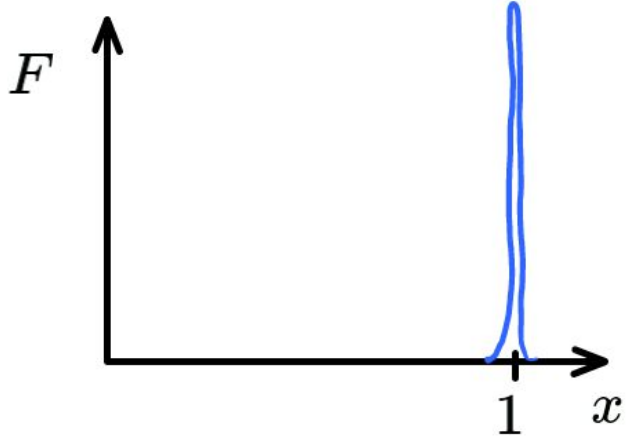
\includegraphics[scale=0.25]{images/DISinelastic1.png}
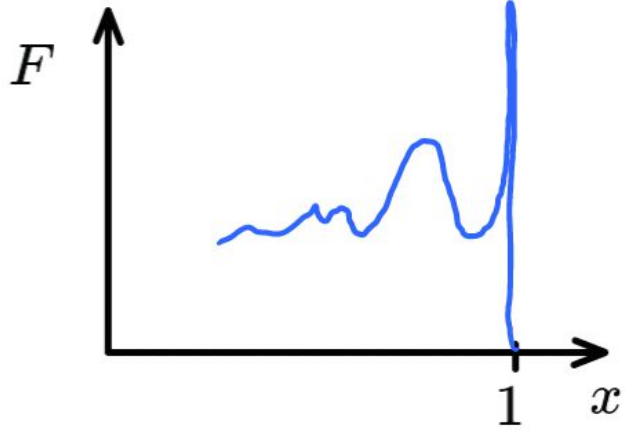
\includegraphics[scale=0.25]{images/DISinelastic2.png}
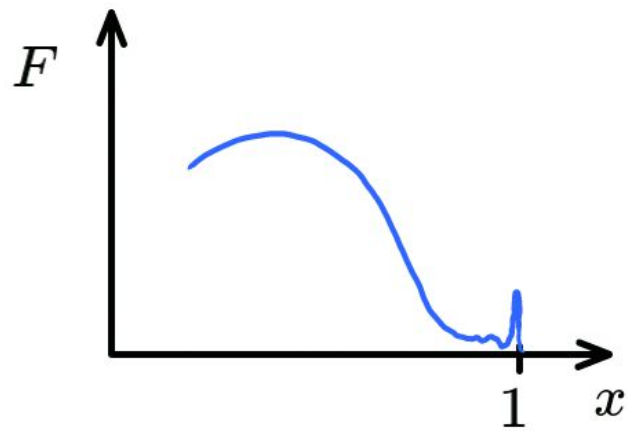
\includegraphics[scale=0.25]{images/DISinelastic3.png}
\end{center}
\caption{Sketch of the form factor behaviour as a function of $x$ for different ranges of $Q^2$.}\label{fig:DISinelastic}
\end{figure}

\begin{figure}[h]
\begin{center}
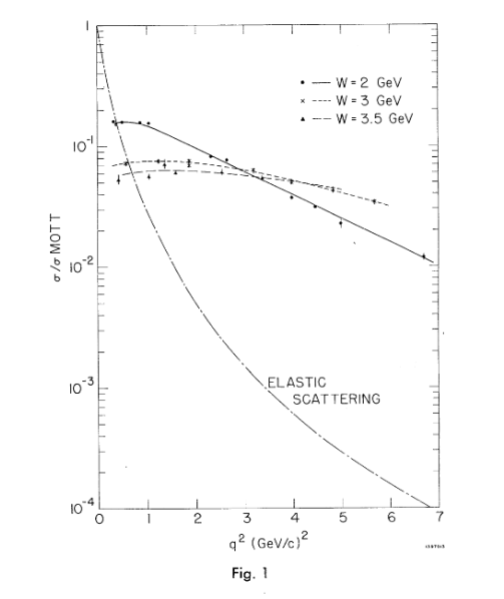
\includegraphics[scale=0.5,trim=1cm 1cm 1cm 1cm]{images/DISq2dep.png}
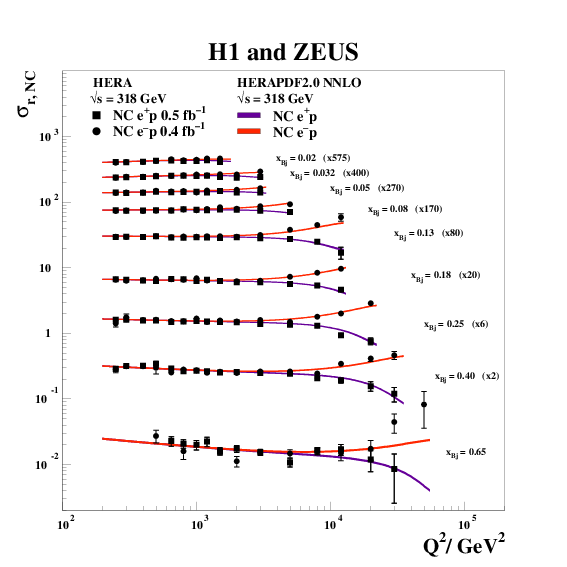
\includegraphics[scale=0.45]{images/HeraStructureFunction.png}
\end{center}
%%\image{HeraStructureFunction.png}
\caption{The left-hand side panel shows the ratio of the measured cross section and Mott cross section in an electron-proton scattering experiment. The dependence Figure from \cite{Breidenbach:1969kd} .The right-hand side panel shows the reduced cross section as a function of $Q^2$ for different values of $x$. The reduced cross section is the cross section divided by the Mott cross section. Each value set of points for a given value of $x$ is shifted to improve readability. The data is from the H0 and Zeus experiments at the Hera collider \cite{Abramowicz:2015mha}.}\label{fig:DISq2dep}
\end{figure}
We can also look at the $Q^2$ dependence of the structure functions. Figure~\ref{fig:DISq2dep} shows the $Q^2$ dependence of the ratio of the measured cross section and the Mott cross section in an electron-proton scattering experiment. If the proton was made up of a uniform charge and magnetic moment density we would expect the ratio to fall off quickly but we find that for high enough values of $Q^2$ the ratio is not falling as fast as we expect. The fact that the structure constants fairly constant indicates that we might have found some point-like structure in the proton! A more convincing plot of the $Q^2$ independence is shown in the right-hand side of Figure~\ref{fig:DISq2dep}
%
%%\lecture{13}
%%\section{The Parton Model}
\clearpage
\subsection{Parton model}
%
%
Given the relative independence of the structure function we are led to think that there is a point-like structure within the nucleon. This is the starting point of the parton model: the nucleon is composed of point-like constituents called partons, and the inelastic scattering with the nucleon is actually an elastic scattering with one of the partons. 
%%\keypoint{The parton model stipulates that the proton is made up from constituent particles called partons (we know now that they are quarks and gluons.}

The kinematics in this model is shown in Figure~\ref{fig:DISkinematics}. The incoming and outgoing electrons have momenta $p$ and $p'$, the proton has momentum $P$ before the scattering and $W$ after scattering. The momentum transferred by the virtual photon is $Q^2=-q^2$. We now assume that the reaction actually takes part between the virtual photon and a parton that carries a fraction $0<\eta<1$ of the momentum of the proton. 
\begin{figure}[h]
\begin{center}
%%\image{DISkinematics.png}
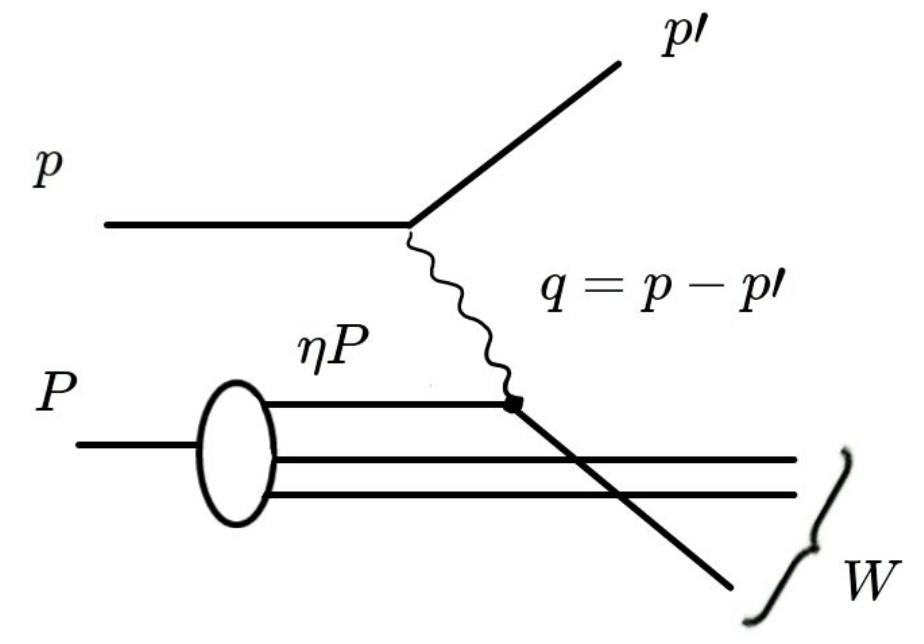
\includegraphics[scale=0.25]{images/DISkinematics.png}
\end{center}
\caption{Kinematics of deep inelastic scattering.}\label{fig:DISkinematics}
\end{figure}
If we assume that the parton is massless we can calculate its momentum fraction $\eta$ by computing the square of the outgoing parton momentum $k$:
\[0=k^2=\left(\eta P+p-p'\right)^2=\left(\eta P+q\right)^2=\eta^2M^2+2\eta P\cdot q-Q^2\]
If we assume that the energies in the process are much larger than the proton mass we can neglect the $M^2$ term and solve for $\eta$:
\[\eta=\frac{Q^2}{2P\cdot q}=x\] 

\begin{wrapfigure}{r}{0.4\textwidth}
\begin{center}
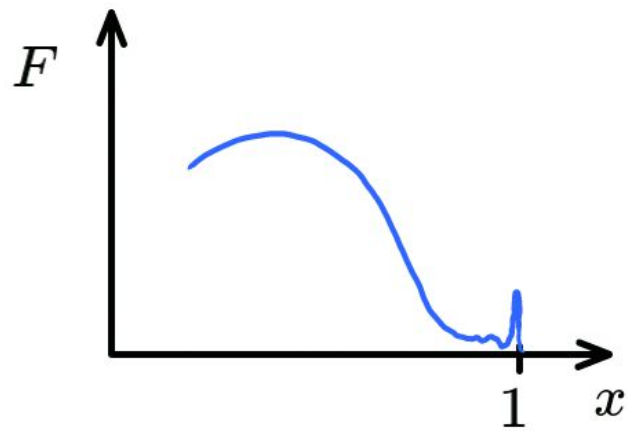
\includegraphics[scale=0.25]{images/DISinelastic3.png}
\end{center}
\end{wrapfigure}
Now we have a more physical interpretation of the kinematical parameter $x$: it is the fraction of the proton momentum carried by the parton that is struck in the scattering. This interpretation is only valid in the limits mentioned above but are applicable in practice. We can now go back to the right-most sketch in Figure~\ref{fig:DISinelastic} and give an interpretation of the peak at $x\simeq 1/3$: it means that we have the highest cross section for a scattering with a parton that carries about a third of the total proton momentum, so we are lead to believe that the proton is composed of three objects.

The $F_1$ and $F_2$ structure functions encapsulate information about the electric and magnetic properties of the constituents of the nucleons. If these constituents are spin $1/2$ particles then there is a relationship between $F_1$ and $F_2$ called the Callan-Gross relation:
\begin{equation}\label{eq:CallanGross}
F_2(x,Q^2)=2xF_1(x,Q^2)\;.
\end{equation} 
Figure~\ref{fig:CallanGross} shows the ration of the left and right-hand side of equation~\ref{eq:CallanGross}. The fact that the data is consistent with the ratio being $1$ is evidence that the constituents of the nucleon are spin $1/2$ particles. These particles are called \emph{quarks} and we an study their properties by studying the structure functions.
\begin{figure}
\begin{center}
%%\image{CallanGross}
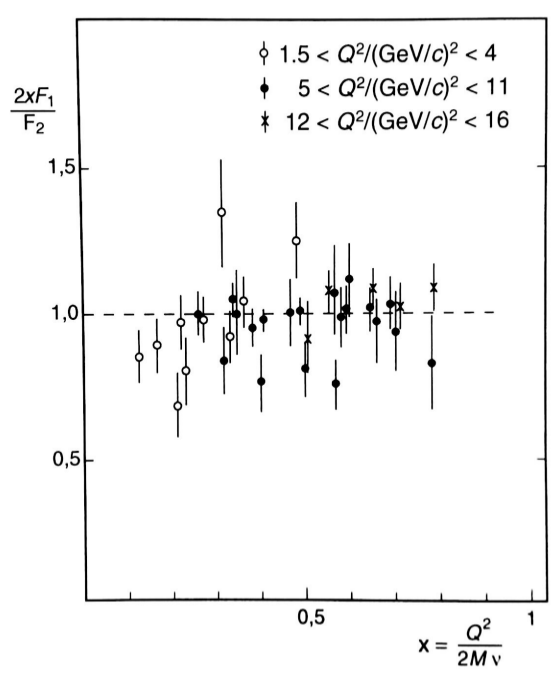
\includegraphics[scale=0.4]{images/CallanGross}
\end{center}
\caption{Ratio of $2xF_1(x)$ and $F_2(x)$ for different values of $Q^2$. Data from SLAC, figure from \cite{povh}.}\label{fig:CallanGross}
\end{figure}
%%\keypoint{The fact that the structure function follows the Callan-Gross relation is a sign that the constituents in the nucleons are spin $1/2$ particles.}
We now have the elements we need to formulate the parton model: the inelastic
scattering cross section if given by the sum of the cross section of the elastic scattering off the constituents
\begin{equation}\label{eq:partonModel}
\frac{d\sigma}{dQ^2\, dx}=\sum\limits_{\mbox{constituents}} f_c(x) \frac{d\sigma}{dQ^2}(e^-,c;p,xP,p') \end{equation}
where $f_c(x)$ is the number density of the constituent $c$, that is the number of partons of type $c$ with momentum fraction in an infinitesimal interval around $x$.
\[dn_c(x)=f_c(s)\,dx\;.\]
$f_c(x)$ is called a parton distribution function and we will discuss them in more detail in section~\ref{sec:pdf}. To simplify the notation it is often written as $c(x)$ instead of $f_c(x)$.

Equation~\ref{eq:partonModel} gives a prediction of the cross section for the parton model, if we compare this to the form in equation~\ref{eq:diffCrossSectionStructureFunction} we get the parton model prediction for the structure functions. Since the structure function can be measured in collider experiment we can learn something about the partons. 

The cross section for the electron scattering off one constituent is proportional to the charge squared of the constituent. One can show (see workshop problem 5) that the structure function $F_2$ is given by:
\[F_2(x)=x\sum\limits_{constituents}Q_c^2f_c(x)\]
where $Q_c$ is the charge of constituent $c$, the sum runs over all charged constituents. 

\subsection{Partons}
In this section we discuss the two types of partons: the quarks and gluons. The facts described here were gathered through deep inelastic scattering experiments and hadron spectroscopy. 
\subsubsection{Quarks}
Quarks are spin $1/2$ fermions. They come in six different types called \emph{flavour}, shown in the table below.
\begin{center}
\begin{tabular}{c|c|c}
symbol& name & charge \\\hline
$u$ & up & $+2/3$   \\
$d$ & down & $-1/3$  \\
$s$ & strange & $-1/3$ \\
$c$ & charm & $+2/3$ \\
$b$ & bottom & $-1/3$ \\
$t$ & top & $+2/3$
\end{tabular}
\end{center}
Each quark has an anti-particle called anti-quark (denoted by a bar above the symbol) with the opposite charge.

The nucleons are composed of three \emph{valence} quarks. The proton is $uud$ quark combination and the neutron is a $udd$ quark combination. They are the most common example of a bound state of three quarks, which are called \emph{baryons}. There are also bound states of a quark and an anti-quark called $mesons$. Both families of particles will be covered in detail in a later chapter.   

The valence quark give the nucleons their overall quantum numbers. One can easily check that the charge of the proton and neutron is given by the sum of the charges of their valence quarks.

The quarks are interacting through the strong force. As the forces in particle physics the force is mediated through the exchange of a virtual particle. The force carrier of the strong interaction is called the gluon and will be discussed in the next section.
%
%
\subsubsection{gluons}
%
%
Gluons are the carriers of the strong force, they play the same role for the strong force as the the photon for the electro-magnetic force. Unlike photons, the gluons also interact with each other, this leads to a different behaviour of the coupling strength of the strong and electro-magnetic force. The gluons have no electric charge so they do not interact with the photons, so they are invisible when we perform our deep inelastic scattering experiment.

\subsubsection{Sea quarks}

The quarks in the proton are held together by the strong force through exchange of gluons. During the exchange the gluon can split into a virtual quark-anti-quark pair. These quarks and anti-quarks, unlike the gluons, are not invisible to the virtual photon emitted by the incoming electron. These quarks always come in pairs and their quantum numbers cancel and therefore do not contribute to the quantum numbers of the nucleon.

%
%
%%\lecture{14}
%
%
\subsection{Parton distribution functions}\label{sec:pdf}
The parton distribution function give the number density of the partons in the proton (there are also PDFs for other baryons or mesons.) The PDFs depend on the fraction $x$ of the proton momentum they are carrying. The PDFs cannot be predicted from first principle but there are theoretical constraints on their integrals. One of them is that the total contribution of the charged quarks should reproduce the quantum numbers of the proton. For example the charge of the proton has to be $1$:
%%\keypoint{The constituents have a momentum fraction distribution described by parton distribution functions.}
\[\int\limits_0^1\sum\limits_{q}Q_qf_q(x)\,dx=1\,.\]
The sum runs over all quarks and anti-quarks only, as gluons have no electric charge. $Q_q$ is the charge of the quark. 
We also want that the sum of all momentum fractions add up to the total momentum of the proton:
\[\int\limits_0^1\sum\limits_{c} x\,f_c(x)\,dx=1\,.\]
Here the sum over $p$ runs over all quarks, anti-quark and gluons as all carry some momentum. 

The quarks found in the proton have two possible origins. First they can be one of the three quarks that give the proton its baryon properties as a $uud$ bound state, these quarks are called valence quarks. Secondly they can be a quark or anti-quark created as part of the cloud of virtual particles surrounding the valence quarks. We distinguish the two types of quarks with a valence PDF and a ``sea'' distribution
\[f_q(x)=f_q^V(x)+f_q^S(x)\;.\]
%%\keypoint{There are two types of quarks in a nucleon: the valence quark that give the quantum numbers of the nucleon and the sea quarks that come in pairs and don't give a net contribution to the quantum numbers of the nucleon.}
To help imagining what the PDFs are it is helpful to think about how they would look like if the structure of the proton was much easier. If there were only the three valence quarks and each of the three quarks carried exactly one third of the momentum of the proton we would get the results of Fig.\ref{fig:pdfab}
\begin{figure}[h]
\begin{center}
	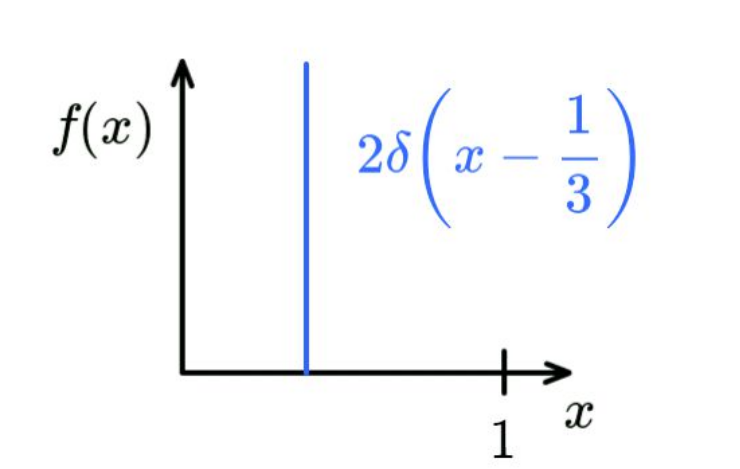
\includegraphics[scale=0.25]{images/PDFa.png}
    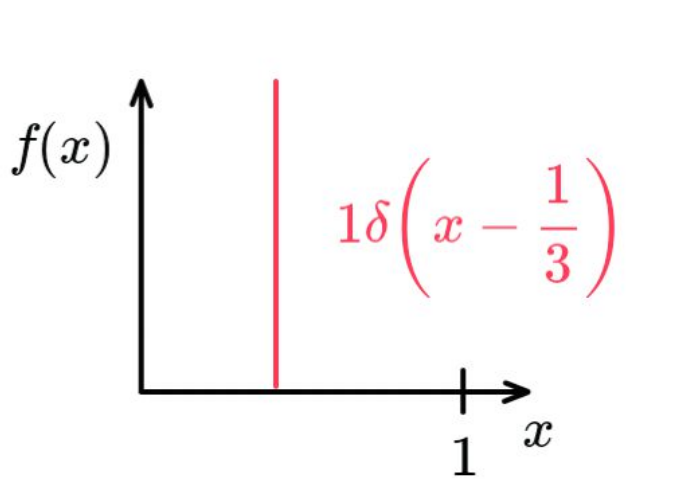
\includegraphics[scale=0.25]{images/PDFb.png}
\end{center}
  \caption{PDF distributions if there were only the three valence quarks and they all had one third of the momentum of the proton. The left-hand plot is for the $u$ quark and the right-had plot for the $d$ quark }
  \label{fig:pdf13}
  \end{figure}
In this case the PDFs would be simple delta functions fixing the momentum fraction to $1/3$. The $u$ PDF is normalised such that it gives $2$ when integrated over $x$, since we have two valence $u$ quarks and the $d$ PDF integrates to $1$. Another example shown in Fig \ref{fig:pdfcd} is in the hypothetical case where we only have valence quarks and the two $u$ quarks have to share half the momentum of the proton and the single $d$ quark carries the other half. The momentum fractions of the $u$ quark are not fixed to $1/4$ as one of the quark can have a larger share of the $1/2$ of the proton momentum as long as the other one. The area under the $u$ PDF curve still has to be equal to he number of valence $u$ quarks.  
\begin{figure}[h]
\begin{center}
  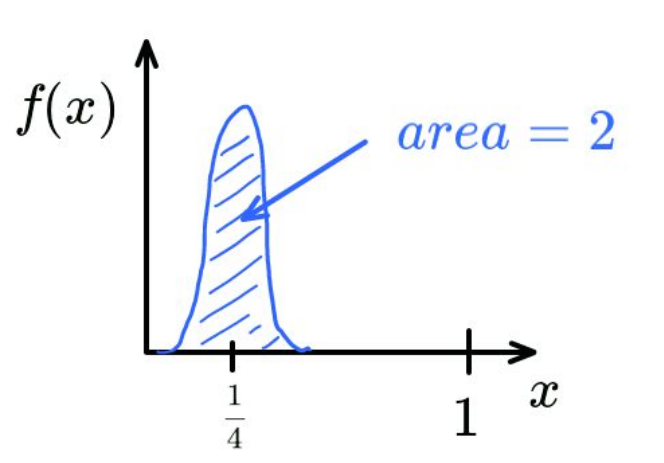
\includegraphics[scale=0.25]{images/PDFc.png}
    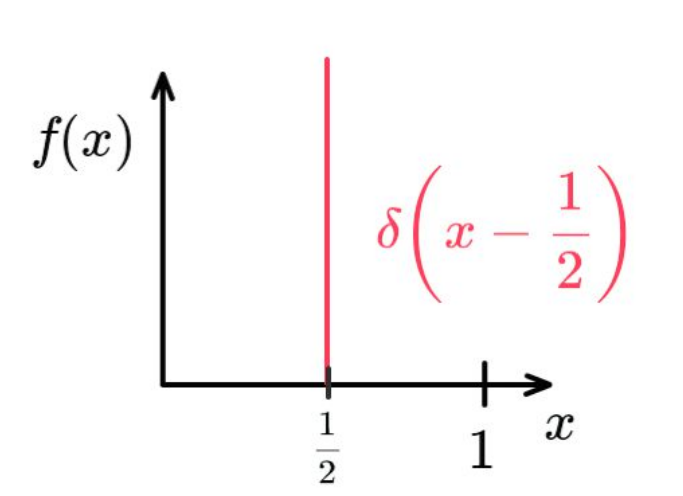
\includegraphics[scale=0.25]{images/PDFd.png}
\end{center}
  \caption{PDF distributions if there were only the three valence quarks and the two $u$ quarks share half of the momentum while the $d$ quark carries the rest of the momentum of the proton. The left-hand plot is for the $u$ quark and the right-had plot for the $d$ quark }
  \label{fig:pdfcd}
  \end{figure}
One can now move to a more general parametrisation. Let us see how a PDF would look like if it is of the form
\[f(x)=x^a(1-x)^b\;,\qquad a,b>0\;.\]
This form has some nice properties. The PDF vanishes for $x\rightarrow 0$, which is what we would expect for valence quarks: it is not very likely that a valence quark carries a very small fraction of the proton's momentum. The PDF also vanishes when $x\rightarrow 1$ which is the limit in which the parton described by the PDF carries all of the momentum of the proton, leaving almost nothing to the other partons.     
\begin{figure}[h]
  \begin{center}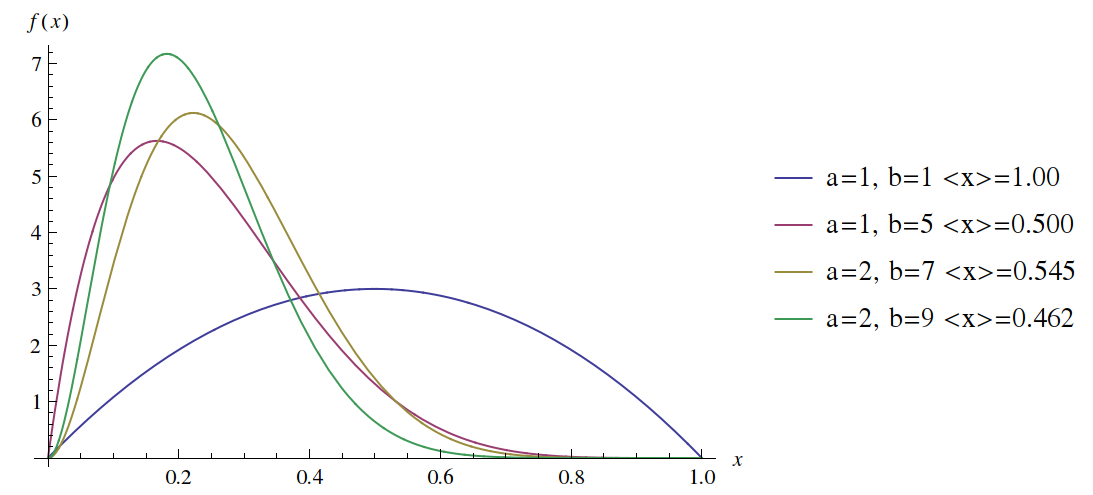
\includegraphics[scale=0.25]{images/PDFs.png}
    \end{center}
  \caption{PDF distributions of the form $x^a(1-x)^b$. The expectation value $\langle x\rangle$ gives the average fraction of the proton momentum a quark with this PDF would carry. }
  \label{fig:pdfab}
  \end{figure}
So far we have focused on the valence quarks. The sea quarks typically carry a small fraction of the proton momentum. Their PDFs vanish very quickly for $x->1$ but do not vanish at $x\rightarrow 0$. The gluons also tend to carry a lower fraction of the proton momentum than the quarks, but their contribution becomes dominant at small values of $x$, as shown in Fig. \ref{fig:pdfMSTW}.

The PDFs cannot be predicted solely by theoretical methods and have to be measured experimentally. The most common method to do so is to create an ansatz such as the one we had above ($f(x)=x^a(1-x)^b$) and fit the parameters ($a$ and $b$ in our example) 
%%\image{plotpaw.png}
\begin{figure}[h]
  \begin{center}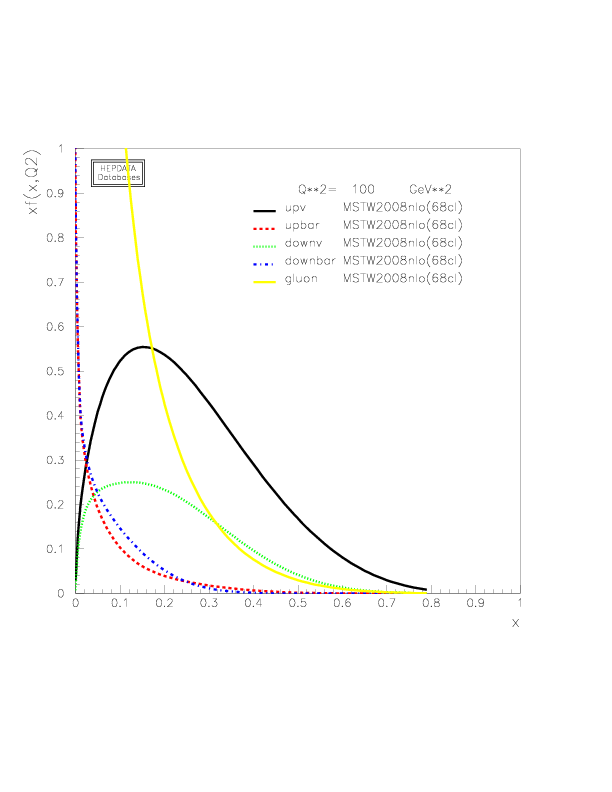
\includegraphics[scale=0.3,trim=20 150 50 120,clip]{images/plotpaw.png}
    \end{center}
  \caption{Actual PDF fit performed by the MSTW group (Martin,Stirling,Thorne,Watt). You can look at the PDFs yourself and make plots at \url{http://hepdata.cedar.ac.uk/pdf/pdf3.html}. It is customary for PDFs to be plotted as $xf(x)$ instead of $f(x)$, This is the quantity that enters the form factor $F_2(x)$.}
  \label{fig:pdfMSTW}
  \end{figure}
%%\section{Quark Structure of the Nucleus}
\subsection{Quark structure of the nucleons}
We now know that the charged constituents are quarks and that we can rewrite the structure function as 
\[F_2(x)=x\sum\limits_{f}Q_f^2(q_f(x)+\bar q_f(x)\;,\]
where the sum runs over the quark flavours. The $c,b,t$ quarks are too heavy to play a significant role in DIS experiments so we can limit the sum to the three lighter quarks $u,d,s$. The neutrons and protons are made up of $u$ and $d$ quarks, but no $s$ quarks, so the $s$ quarks only appear in the sea quark distribution. Separating each quark parton distribution function into a valence and a sea contribution we can write down the structure function for the scattering of an electron off a proton:
\begin{eqnarray*}\label{eq:F2ep}
F_2^{e,p}(x)&=&x\sum\limits_{f=u,d,s}Q_f^2(q_f(x)+\bar q_f(x))\\
&=&x\left[
\frac{1}{9}\left(d_V^p+d_S^{p}+\bar d_S^p\right)+
\frac{4}{9}\left(u_V^p+u_S^{p}+\bar u_S^p\right)+
\frac{1}{9}\left(s_S^{p}+\bar s_S^p\right)
\right]\;,
\end{eqnarray*}
where the argument $x$ of the distributions $q_f(x)$A has been omitted for readability. A proton and a neutron differ by the fact that the roles of the $u$ and $d$ quarks are inverted. We will see later that the relative similarity of the proton and neutron, called isospin symmetry, is a useful tool to understand the structure of baryons. Here we will only use the approximate symmetry between the neutron and the proton to argue that the distributions of $u$ in the proton and $d$ in the neutron should be the same, and reciprocally.
\[u_V^p\simeq d_V^n\;, d_V^p\simeq u_V^n\;, s_S^p(x)\simeq s_S^{n}(x)\;.\] 
Using this approximation we can write the expression for the structure function for the electron scattering off a neutron.  
\begin{eqnarray*}\label{eq:F2en}
F_2^{e,n}(x)&=&x\left[
\frac{1}{9}\left(d_V^n+d_S^{n}+\bar d_S^n\right)+
\frac{4}{9}\left(u_V^n+u_S^{n}+\bar u_S^n\right)+
\frac{1}{9}\left(s_S^{n}+\bar s_S^n\right)
\right]\\
&=&x
\left[
\frac{1}{9}\left(u_V^p+u_S^{p}+\bar u_S^p\right)+
\frac{4}{9}\left(d_V^n+d_S^{p}+\bar d_S^p\right)+
\frac{1}{9}\left(s_S^{p}+\bar s_S^p\right)
\right]\;,
\end{eqnarray*}
where we have used the above approximation to rewrite the neutron parton distributions in terms of the proton ones. If our target consists of and equal amount of protons and neutron, we can measure the average nucleon structure function bu averaging equations (\ref{eq:F2ep}) and (\ref{eq:F2en}):
\begin{eqnarray*}\label{eq:F2eN}
F_2^{e,N}(x)&=&\frac{F_2^{e,p}+F_2^{e,n}}{2}=x\left[
\frac{5}{18}\left(d_V^n+d_S^{n}+\bar d_S^n\right)+
\frac{5}{18}\left(u_V^n+u_S^{n}+\bar u_S^n\right)+
\frac{1}{9}\left(s_S^{n}+\bar s_S^n\right)
\right]\;.
\end{eqnarray*}
If we change the incoming particle instead of the target we can also calculate the structure function for the scattering of a neutrino with nucleons. This time the interaction is the weak interaction instead of the electro-magetic force. 
%%\keypoint{We can get information about the parton distribution functions using DIS with different targets and using electrons or neutrinos in the collision.}

The structure function is given by
\begin{equation}\label{eq:F2vN}
F_2^{\nu,N}=x\sum\limits_f\left(q_f(x)+\bar q_f(x)\right)\;.
\end{equation} 
If we neglect the $s$-quark contribution we find 
\[\frac{F_2^{2,N}(x)}{F_2^{nu,N}}=\frac{5}{18}\;.\]
This result is confirmed by the experiment, as shown in figure~\ref{fig:F2vN}.
\begin{figure}
%%\image{neutrinoNucleonStructureFunction.png} 
\begin{center}
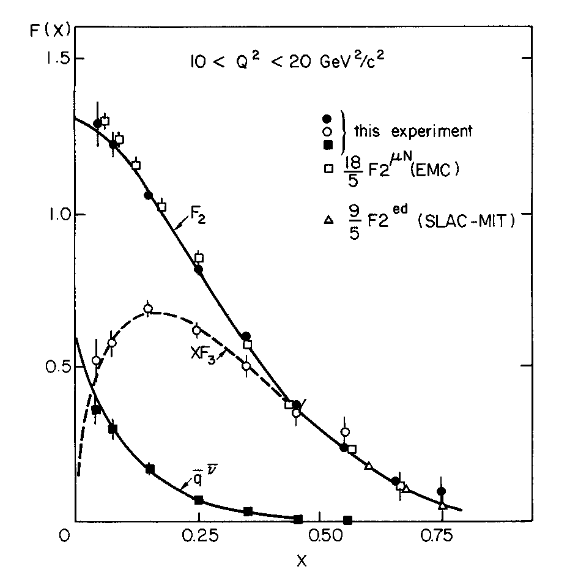
\includegraphics[scale=0.5]{images/neutrinoNucleonStructureFunction.png} 
\end{center}
\caption{Structure functions $F_2$. The figure shows the structure functions for different beams and targets. The figure also shows $xF_3$ which is a measure of the valence quark distribution and the $\bar q$ distribution which is related to the sea quark distribution. The figure is taken from the original data publication \cite{Abramowicz:1982re}.}\label{fig:F2vN}
\end{figure}
\subsubsection{Momentum distribution} 
We have seen that the parton distribution functions $f_c(x)$ give the probability of finding a parton with a momentum fraction $x$ of the proton momentum $P$. We can estimate the momentum $p_f$ carried by the quarks and anti-quarks of flavour $f$:
\[p_f=\int\limits_0^1dx\;\left(q_f(x)+\bar q_f(x)\right)\,xP\;.\]
So the fraction of the total proton momentum carried by the quarks is given by
\[\frac{\sum_f p_f}{P}=\int\limits_0^1 dx\, x \left(q_f(x)+\bar q_f(x)\right)=\int\limits_0^1 dx\, F_2^{\nu,N}(x)=\frac{18}{5} \int\limits_0^1 dx\,F_2^{e,N}(x)\;.\]   
If there were only quarks and anti-quarks in the proton we would expect this fraction to be $1$ but experimentally it is found to be close to $0.5$, so we can conclude that there are other partons in the proton that do not interact either electro-magnetically (with the electrons) or weakly (with the neutrinos). These particles are the gluons.   
%%\keypoint{The total momentum fraction carried by the quarks in a nucleon is about 1/2. Which means that the rest should be carried by particles with no electric of weak charges. The rest of the momentum is carried by the gluons.}
%
%
\subsection{Colour}
%
%
The $u$, $d$ and $s$ quarks were originally introduced as a theoretical device to help understanding the properties of the baryons (as we will see in a later section), Only later were they discovered to actually correspond to actual particles. 

One of the baryons is the $\Delta^{++}$ resonance, it has charge $+2$ and is composed of three valence $u$ quarks. It has a spin of $3/2$ and has positive parity. With our current understanding of the quarks we run into difficulties to describe the $\Delta^{++}$ wave-function: we have the following constraints on the wave function
\begin{itemize}
\item Since we have spin $3/2$ all $3$ spins $1/2$ of the quarks have to be aligned, so the spin wave function has to be symmetric
\item Since the three valence quarks are $u$ quarks the flavour part of the wave function has to be symmetric
\item The $\Delta^{++}$ resonance is the lightest spin $3/2$ baryon so the most likely orbital wave function is one with no orbital angular momentum between the valence quark. Such a wave function is symmetric   
\end{itemize} 
All these constraints imply that the wave function of the $Delta^{++}$ resonance is fully symmetric, but this is in contradiction with the Pauli exclusion principle that states that a state made up of fermions (and $u$ quarks are fermions) should be anti-symmetric with respect to the exchange of any two identical fermion. This problem can be resolved by adding a quantum number to the quarks such that their state can be anti-symmetric with respect to that quantum number and therefore overall anti-symmetric with respect to the exchange of two quarks. 

%%\keypoint{We need to introduce a new quantum number to accommodate for the $\Delta^{++}$ resonance in order to respect the Pauli exclusion principle.}

The quantum number we introduce is called the \emph{colour}. The colour charge can take on three different values that we call red, green or blue and denote with $r$, $g$ and $b$. Anti-quark carry anti-colour charges denoted as $\bar r$, $\bar g$ and $\bar b$. The strong force is the interaction between colour charges and is carried by the gluons. It turns out that the gluons also carry colour charges, namely a colour-anticolour combination, for example $r\bar g$, $b\bar r$...    
%%\keypoint{Quarks and gluons carry colour charges. Quarks can have one of three colours, antiquarks carry anti-colour charges and gluons carry a colour-anticolour charge.}

The interaction with the gluon changes the colour of the quark, as illustrated in figure~\ref{fig:colour}. Since the gluons carry colour charges they can also interact with themselves. The colour exchanges in such an interaction is illustrated in figure~\ref{fig:colour}. The fact that this interaction makes the strong interaction very different from the the electro-magnetic force. 

While the electro-magnetic interaction is \emph{screening}, that is vacuum fluctuations tend to shield the electric charge. The farther one is from a charge the smaller its effective charge appears. The main effect being that as one increases the resolution of the scattering experiment the virtual photon penetrates more and more into the cloud of virtual particles-antiparticles that surround the charge, revealing a larger and larger charge. The net effect is that the electro-magnetic coupling strength is increasing as the energy increases. 
%%\keypoint{Gluons are the carriers of the strong interaction. Since gluons also carry colour charges, they can interact between themselves, which photons cannot. One consequence is that the strong coupling is increasing as the energy lowers (which means that the distance increases).}

On the contrary the strong force is \emph{anti-screening}. The strength of the interaction increases with the distance. One dramatic consequence is that colour charged particles cannot be observed in isolation: to separate two colour charges it would take an infinite amount of energy, and before this is reached a colour-anticolour pair can be created from the vacuum, so that we never manage to create a large distance between colour charges. This is illustrated below.
%%\keypoint{Only colour neutral objects can exist at a scale of $\simeq  1$ fm. }

\begin{figure}
\begin{center}
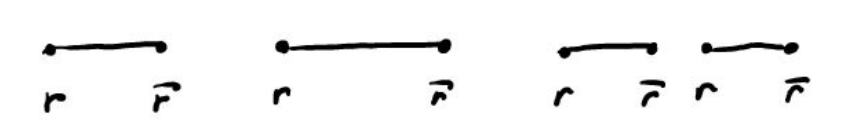
\includegraphics[scale=0.45]{images/hadronisation.png}
\end{center}
\caption{Illustration of the process through which color neutral particles are created.}\label{fig:hardonisation}\end{figure}
 The experimental consequence is that only globally colour neutral particles can be observed.      
%%\image{GluonColor.png}
\begin{figure}
\begin{center}
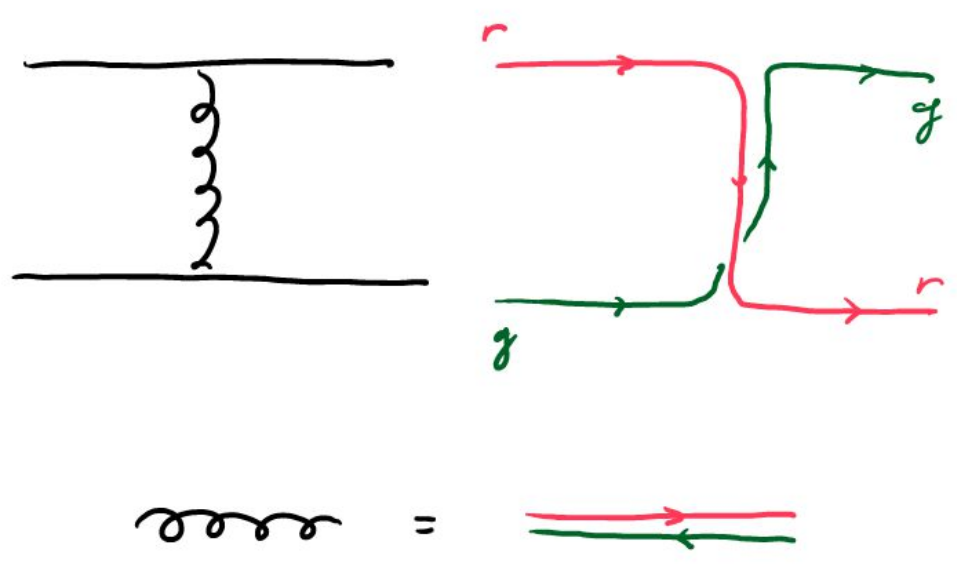
\includegraphics[scale=0.35]{images/ColorExchange.png}
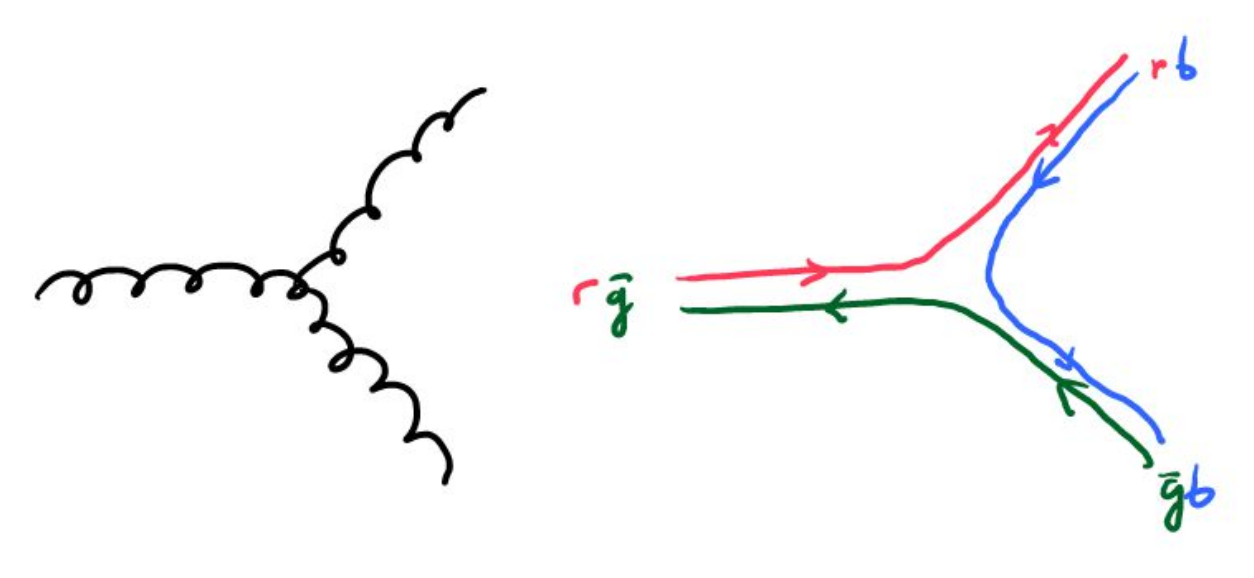
\includegraphics[scale=0.25]{images/GluonColor.png}
\end{center}
\caption{Colour flow for the interaction of a gluon and two quarks (above) and for three gluons (below).}\label{fig:colour}
\end{figure}

%%\lecture{15}

%
%%\section{Scaling Violation}
\subsection{Scaling violation}
%
The PDFs also exhibit a $Q^2$ dependence, this can be understood by the fact that resolving the proton structure in finer detail (the ``resolution'' of the photon is increasing as $Q^2$ is increasing) reveals more sea quarks and gluons than at a lower resolution, and hence the exact composition of the proton depends on the resolution scale we are probing it at. 
%%\keypoint{The parton distribution functions have a mild energy dependence, this is due to the fact that at a larger energy we can resolve more of the cloud of sea quarks and gluons present in the nucleon.}
%%\image{Q2depPDF.png}
\begin{figure}
\begin{center}
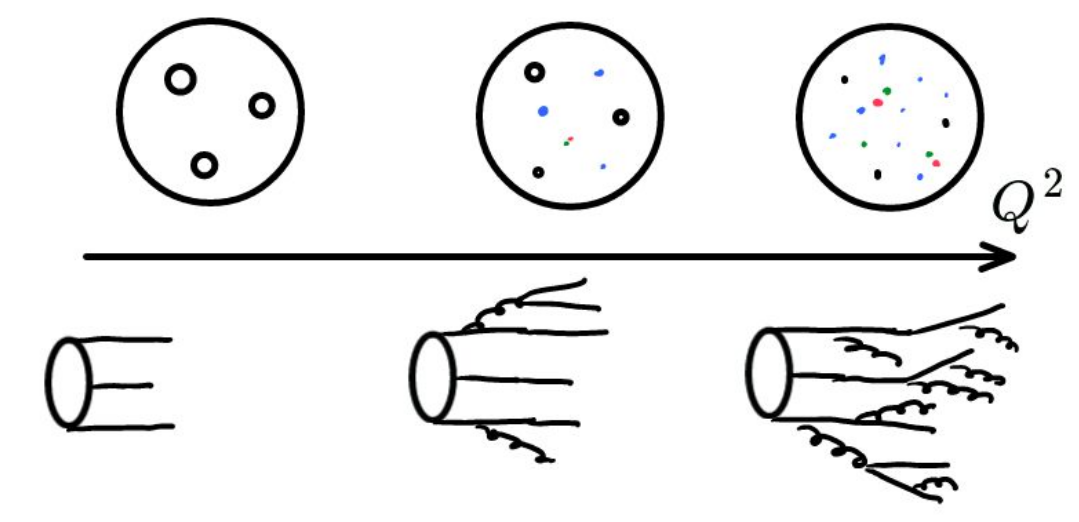
\includegraphics[scale=0.3]{images/Q2depPDF.png}
\end{center}
\caption{Illustration of the $Q^2$ dependence of the parton distribution function. As the resolution increases the virtual proton can resolve more and more of the interactions that happen inside the quark bound state that is the proton. On the left, when the energy is quite small one can only resolve the three valence quarks. In the middle part of the diagram the energy is sufficient to resolve some of the quarks and some of the sea quarks. In the right of the diagram the energy is high enough to see more and more sea quarks and gluons.}\label{fig:Q2depPDF}
\end{figure}

\clearpage
\section{Key Points}
\begin{itemize}
\item The cross section is a very useful quantity to characterise a physical scattering process.
\item More information about the dynamics of the interaction can be shown by measuring the cross section differentially with respect to observables. Such a differential cross section is represented as an histogram.
\item The Rutherford cross section describes the elastic scattering of a charged particle off the potential created by another charge.
\item When the projectile is relativistic, its spin has to be taken into account, this leads to the Mott cross section.
\item Helicity conservation suppresses backward scattering.
\item If the scattering is off a charge distribution instead of a point-particle then the matrix element is reduced by a factor called the form factor. The form factor is the Fourier transform of the charge distribution. The cross section is reduced by the square of the magnitude of the form factor.
\item Looking at the ratio between the point-like cross section and the actual cross section one can infer the form of the charge distribution. Using this technique one can measure the charge distribution in the nucleus of an atom.
\item One can use the same technique to measure the charge distribution of the proton or neutron. In this case we need to consider the magnetic interaction due to the spin of the nucleon and one can measure both the electric charge and the magnetic moment distribution inside the nucleons.
\item If the energy is further increased the proton is changed after the scattering and the scattering is therefore non-elastic. As a consequence we now need two parameter to describe the scattering. 
\item Because we are now able to create and destroy states we need to go from Quantum Mechanics to Quantum Field Theory. One consequence is that fores are now mediated through the exchange of a particle.
\item In a deep inelastic experiment one collides a large energy electron with a proton.
\item At low energies one sees an elastic scattering of the electron off the proton.
\item At moderate energies the electron can transfer enough energy to excite the nucleon to excited states (some of them are the $\Delta$ baryons).
\item At higher energies the electron recoils against point-like objects inside the proton.
\item These constituents are spin $1/2$ particles.
  \item The parton model stipulates that the proton is made up from constituent particles called partons (we know now that they are quarks and gluons) 
  \item The constituents have a momentum fraction distribution described by parton distribution functions.
    \item There are two types of quarks in a nucleon: the valence quark that give the quantum numbers of the nucleon and the sea quarks that come in pairs and don't give a net contribution to the quantum numbers of the nucleon.
  \item We can get information about the parton distribution functions using DIS with different targets and using electrons or neutrinos in the collision.
  \item The total momentum fraction carried by the quarks in a nucleon is about 1/2. Which means that the rest should be carried by particles with no electric of weak charges.
  \item We need to introduce a new quantum number to accommodate for the $\Delta^{++}$ resonance.
  \item Quarks and gluons carry colour charges. Quarks can have one of three colours, antiquarks carry anti-colour charges and gluons carry a colour-anticolour charge.
  \item Gluons are the carriers of the strong interaction. Since gluons also carry colour charges, they can interact between themselves, which photons cannot. One consequence is that the strong coupling is increasing as the energy lowers (which means that the distance increases)
  \item Only colour neutral objects can exist at a scale of $\simeq \, 1\,\rm{fm}$.
    \item The parton distribution functions have a mild energy dependence, this is due to the fact that at a larger energy we can resolve more of the cloud of sea quarks and gluons present in the nucleon.
\end{itemize}
\subsection{Quick questions}
\begin{itemize}
\item What are the parameters affecting the luminosity of an experiment.
\item What is the difference for the differential cross section $d\sigma/dq^2$ if the target is point-like or has a spatial extent.
\item How does one estimate the radius of a nucleus?
\item What evidence do we have that protons and neutrons are not point-like particles? 
\item Can you explain the different type of behaviour of the scattering at different energies in  terms of the wavelength of the exchanged photon?
\item How do we know that in DIS the electrons recoil against point-like particles?
\item How do we know that the constituents struck in DIS are spin $1/2$ particles?
\item How would the parton distribution functions look like if the three valence quarks were sharing the proton's momentum equally?
\item How do we know that the total momentum fraction carried by the quarks in a nucleon is about 1/2?
\item How do the valence quark and the sea quark parton distribution look like as a function of the momentum fraction $x$?
\item What does isospin symmetry say about the $u$ and $d$ parton distribution functions in the proton and neutron?
\item How many colour states of gluons are there?
  \item The colour charges are conserved, can you draw the flow of the colour charges in a 3-gluon vertex and in a diagram of the scattering of two quarks?
\end{itemize}
%
%
%
%
%
%
%
%
%%\section{Appendix}
\clearpage
\appendix
\section{Direct Fourier transform of the EM potential}
so that we get for the matrix element
\[\mathcal{M}_{fi}=\left<\psi_f|\mathcal{H}_{int}|\psi_i\right>
=e\int dx\,\psi_f^*(x)\phi(x)\psi_i(x)\;.
=\frac{e}{V}\int dx\,e^{-i\V{p'}\cdot x}\phi(x)e^{i\V{p}\cdot\V{x}}
=\frac{e}{V}\int dx\,e^{i\V{q}\cdot x}\phi(x)\;.
\]
where we used the momentum transfer $\V{q}=\V{p}-\V{p'}$. There are different ways of proceeding from here, see ch. 5.2 of the book for a different way. To calculate the matrix element we first consider a simpler example where the charge distribution is point-like, and therefore the potential takes the usual $1/r$ form of the Coulomb potential. 
\[\rho(x)=ze\delta^{3}(\V{x}-\V{x}_0)\;,\quad \phi(x)=\frac{Ze}{\left|\V{x}-\V{x}_0\right|}\] 
Inserting this in the matrix element calculation yields
\begin{eqnarray*}
\mathcal{M}_{fi}&=&\left<\psi_f|\mathcal{H}_{int}|\psi_i\right>
=\frac{e}{V}\int d^3x\,e^{i\V{q}\cdot x}\phi(x)
=\frac{e}{V}\int d^3x\,e^{i\V{q}\cdot x}\frac{Ze}{\left|\V{x}-\V{x}_0\right|}
\;.
\end{eqnarray*}
We now change variable to $\V{x'}=\V{x}-\V{x}_0$ introduce polar coordinates for the  $\V{x}_0$ integration. We can choose the $z$ axis to be along the direction on $\V{q}$, so we get
\begin{eqnarray*}
  \mathcal{M}_{fi}&=&\frac{e}{V}\int d^3x\,e^{i\V{q}\cdot x}\frac{Ze}{\left|\V{x}-\V{x}_0\right|}
  =\frac{e^2Z}{V}\int d^3x'\,e^{i\V{q}\cdot \V{x_0}}\,e^{i\V{q}\cdot \V{x'}}\frac{1}{\left|\V{x'}\right|}\\
  &=&\frac{e^2Z}{V}e^{i\V{q}\cdot \V{x_0}}2\pi\int\limits_0^\infty r^2\, dr\int\limits_{-1}^{1}d\cos\theta \,e^{i|\V{q}|r\cos\theta}\,\frac{1}{r}
  =\frac{2\pi e^2Z}{V}e^{i\V{q}\cdot \V{x_0}}\int\limits_0^\infty r\, dr\left. \frac{1}{i|\V{q}|r}e^{i|\V{q}|r\cos\theta}\right|_{\cos\theta=-1}^{\cos\theta=+1}\\
  &=&\frac{2\pi e^2Z}{V}e^{i\V{q}\cdot \V{x_0}}\int\limits_0^\infty \, dr \frac{1}{i|\V{q}|}\left(e^{i|\V{q}|r}-e^{-i|\V{q}|r}\right)=\frac{2\pi e^2Z}{i|\V{q}|V}e^{i\V{q}\cdot \V{x_0}} \left. \left(\frac{e^{i|\V{q}|r}}{i|\V{q}|}-\frac{e^{-i|\V{q}|r}}{-i|\V{q}|}\right)\right|_0^\infty
  \\
  &=&
  \frac{2\pi e^2Z}{i|\V{q}|V}e^{i\V{q}\cdot \V{x_0}} \left. \left(\frac{e^{i|\V{q}|r}}{i|\V{q}|}-\frac{e^{-i|\V{q}|r}}{-i|\V{q}|}\right)\right|_0^\infty= \lim\limits_{R\rightarrow \infty}\frac{2\pi e^2Z}{|\V{q}|^2V}e^{i\V{q}\cdot \V{x_0}}\left(2-2\cos(|\V{q}|R)\right)
\end{eqnarray*}

This is problematic since the term at infinity is undetermined. One could argue that it has to vanish as the boundary condition on $q$ for a particle in volume $V$, but it is not straight-forward. 

\bibliographystyle{ieeetr}
\bibliography{bibliography}
 


\end{document}


